\section{Discrete Random Variables}
\emph{Motivation}: Roll two dice.
$\Omega = \{1, \dots, 6\}^2 = \{(i, j) : 1 \leq i, j \leq 6\}.$
If we restrict our attention to:
\begin{itemize}
    \item the first dice e.g. $\{(i, j) : i = 3\}$.
    \item the sum of the dice e.g. $\{(i, j) : i + j = 8\}$.
    \item the max of the dice e.g. $\{(i, j) : i, j \leq 4, i \text{ or } j = 4\}$.
\end{itemize} 
This is annoying and we want to move on from sets.

\emph{Goal}: ``Random real-valued measurements'', we want the value of the first dice to be $X$ and the sum to be $X + Y$\dots

\begin{definition}[Discrete Random Variable]
    A \vocab{discrete random variable} $X$ on a probability space $(\Omega, \mathcal{F}, \mathbb{P})$ is a function $X : \Omega \to \mathbb{R}$ \color{blue} s.t. 
    \begin{itemize}
        \item $\{ \omega \in \Omega : X(\omega) = x\} \in \mathcal{F}$
        \item $\operatorname{Image}(X)$ if finite or countable (subset of $\mathbb{R}$).
    \end{itemize}
    \color{red} 
    \begin{itemize}
        \item We abbreviate $\{ \omega \in \Omega : X(\omega) = x\}$ as $\{X = x\}$. So $\mathbb{P}(X = x)$ is valid.
        \item Often $\operatorname{Image}(X) = \mathbb{Z}$ or $\mathbb{N}_0$ or $\{0, 1\}$ etc. \emph{not} $\{\text{Heads or Tails}\}$. 
    \end{itemize} \color{black}
    If $\Omega$ is finite or countable and $\mathcal{F} = \mathcal{P}(\Omega)$ both blue bullet points hold automatically.
\end{definition} 

\begin{example}[Part II Applied Probability] \mbox{}
    {\par \centering 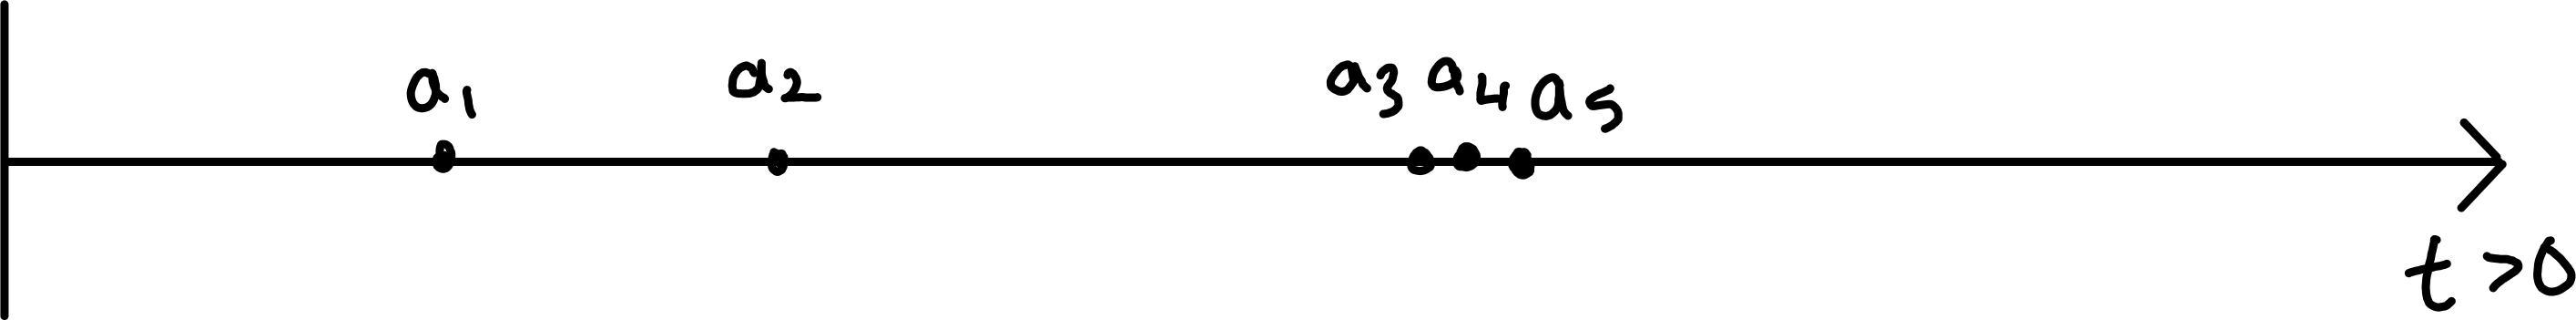
\includegraphics[height=5cm]{04-queue} \par}
    ``random arrival process''.
    Let $\Omega = \{\text{countable subsets } (a_1, a_2, \dots) \text{ of } (0, \infty)\}$ and $N_t =$ number of arrivals by time $t = |\{a_i : a_i \leq t\}| \in \mathbb{N}_0$ is a discrete RV (random variable) for each time $t$.
\end{example} 

\begin{definition}[Probability Mass Function]
    The \vocab{probability mass function} of discrete RV $X$ is the function $p_X : \mathbb{R} \to [0, 1]$ given by $p_X(x) = \mathbb{P}(X = x) \quad \forall \; x \in \mathbb{R}$.
\end{definition} 

\begin{note} \mbox{}
    \begin{itemize}
        \item if $x \notin \operatorname{Image}(X)$ then $p_X(x) = \mathbb{P}(\{\omega \in \Omega : X(\omega) = x\}) = \mathbb{P}(\emptyset) = 0$.
        \mathitem
        \begin{align*}
            \sum_{x \in \operatorname{Im}(X)} p_X(x) &= \sum_{x \in \operatorname{Im}(X)} \mathbb{P}(\underbracket{\{\omega \in \Omega : X(\omega) = x\}}_{\color{blue} \text{disjoint}}) \\
            &= \mathbb{P}\left(\bigcup_{x \in \operatorname{Im}(X)} \{\omega \in \Omega : X(\omega) = x\} \right) \\
            &= \mathbb{P}(\Omega) \\
            &= 1
        \end{align*} 
    \end{itemize} 
\end{note} 
 
\begin{example}[Indicator function]
    For event $A \in \mathcal{F}$, define $1_A : \Omega \to \mathbb{R}$ by 
    \begin{align*}
        1_A(\omega) &= \begin{cases}
            1 & \text{if } \omega \in A \\
            0 & \text{else }
        \end{cases}  
    \end{align*} 
    $1_A$ is a discrete RV with $\operatorname{Image} = \{0, 1\}$.
    $p_{1_A}(1) = \mathbb{P}(1_A = 1) = \mathbb{P}(A)$, $p_{1_A}(0) = \mathbb{P}(1_A = 0) = \mathbb{P}(A^c)$ and $p_{1_A}(x) = 0 \quad \forall \; x \notin \{0, 1\}$.

    \color{blue} This encodes ``did $A$ happen'' as a real number.
\end{example} 

\begin{remark}
    Given a pmf $p_X$ (probability mass function), we can always construct a probability space $(\Omega, \mathcal{F}, \mathbb{P})$ and a RV defined on it with this pmf.

    \color{blue}
    \begin{itemize}
        \item $\Omega = \operatorname{Im}(X)$ i.e. $\{x \in \mathbb{R} : p_X(x) > 0\}$
        \item $\mathcal{F} = \mathcal{P}(\Omega)$
        \item $\mathbb{P}(\{x\}) = p_X(x)$ and extend to all $A \in \mathcal{F}$
    \end{itemize} 
\end{remark} 

\subsection{Discrete Probability Distributions}

\subsubsection{Finite $\Omega$}

\begin{definition}[Bernoulli Distribution - ``(biased) coin toss"]
    If $X \sim \operatorname{Bern}(p)$ where $p \in [0, 1]$ then $\operatorname{Im}(X) = \{0, 1\}$, $p_X(1) = \mathbb{P}(X = 1) = p$ and $p_X(0) = 1 - p$.
\end{definition} 

\begin{example}
    $1_A \sim \operatorname{Bern}(p)$ with $p = \mathbb{P}(A)$.
\end{example} 

\begin{definition}[Binomial Distribution]
    If $X \sim \operatorname{Bin}(n, p)$ where $n \in \mathbb{Z}^+$ and $p \in [0, 1]$ then $\operatorname{Im}(X) = \{0, 1, \dots, n\}$, $p_X(k) = \mathbb{P}(X = k) = \binom{n}{k} p^k (1- p)^{n -k}$.
    $\sum_{k=0}^{n} p_X(k) = (p + (1-p))^n = 1$.
\end{definition} 

The binomial distribution can be used to model the number of heads when a coin is tossed $n$ times.

\subsubsection{More than one RV}

\emph{Motivation}: Roll a dice with outcome $X \in \{1, 2, \dots, 6\}$.
Events: $A = \{1 \text{ or } 2\}$, $B = \{1 \text{ or } 2 \text{ or } 3\}$, $B = \{1 \text{ or } 3 \text{ or } 5\}$.
$1_A \sim \operatorname{Bern}\left(\frac{1}{3}\right)$, $1_B \sim \operatorname{Bern}\left(\frac{1}{2}\right)$, $1_C \sim \operatorname{Bern}\left(\frac{1}{2}\right)$.\\
\emph{Note}: $1_A \leq 1_B$ for all outcomes \\
but $1_A \leq 1_C$ for all outcomes \emph{is false}.

\begin{definition}[Independent RVs]
    Let $X_1, \dots, X_n$ be discrete RVs.
    We say $X_1, \dots, X_n$ are \emph{independent} if:
    \begin{align*}
        \mathbb{P}(X_1 = x_1, \dots, X_n = x_n) &= \mathbb{P}(X_1 = x_1) \dots \mathbb{P}(X_n = x_n) \quad \forall \; x_1, \dots, x_n \in \mathbb{R}.
    \end{align*} 
    \color{blue} (suffices to check $\forall \; x_i \in \operatorname{Im}(X_i)$)
\end{definition} 

\begin{example}
    $X_1, \dots, X_n$ independent RVs each with the Bernoulli(p) distribution.
    Study $S_n = X_1 + \dots + X_n$.
    Then 
    \begin{align*}
        \mathbb{P}(S_n = k) &= \sum_{\substack{x_1 + \dots + x_n = k \\ x_i \in \{0, 1\} }}\mathbb{P}(X_1 = x_1, \dots, X_n = x_n) \\
        &= \sum_{x_1 + \dots + x_n = k} \mathbb{P}(X_1 = x_1) \dots \mathbb{P}(X_n = x_n) \\
        &= \sum_{x_1 + \dots + x_n = k} p^{|\{i : x_i = 1\}|} (1 - p)^{|\{i : x_i = 0\}|} \\
        &= \sum_{x_1 + \dots + x_n = k} p^k (1-p)^{n - k} \\
        &= \binom{n}{k} p^k (1-p)^{n - k}.
    \end{align*} 
    So $S_n \sim \operatorname{Bin}(n, p)$.
\end{example} 

\begin{example}[Non-example]
    $(\sigma(1), \sigma(2), \dots, \sigma(n))$ a uniform permutation.
    \begin{claim}
        $\sigma(1)$ and $\sigma(2)$ are \emph{not} independent.
    \end{claim} 
    Suffices to find $i_1, i_2$ s.t. $\mathbb{P}(\sigma(1) = i_1, \sigma(2) = i_2) \neq \mathbb{P}(\sigma(1) = i_1) \mathbb{P}(\sigma(2) = i_2)$.
    E.g. $\mathbb{P}(\sigma(1) = 1, \sigma(2) = 1) = 0 \neq \underbracket{\mathbb{P}(\sigma(1) = 1) \mathbb{P}(\sigma(2) = 1)}_{= 1 / n \times 1 /n}$
\end{example} 

\underline{Consequence of definition}

Let $X_1, \dots, X_n$ be independent.
Then $\mathbb{P}(X_1 \in A_1, \dots, X_n \in A_n) = \mathbb{P}(X \in A_1) \dots \mathbb{P}(X_n \in A_n) \quad \forall \; A_1, \dots, A_n \subset \mathbb{R}$ countable.

\subsubsection{$\Omega = \mathbb{N}$ - ``Ways of choosing a random integer"}

\begin{definition}[Geometric Distribution (``Waiting for success'')]  
    If $X \sim \operatorname{Geo}(p)$ where $p \in (0, 1)$.
    $\operatorname{Im}(X) = \{1, 2, \dots\}$, \\
    $p_X(k) = \mathbb{P}(\text{(k-1) failures, then success on the kth trial}) = (1-p)^{k-1}p$.
    \color{blue} Check: $\mathcolor{blue}{\sum_{k \geq 1} (1-p)^{k - 1} p = p \sum_{t \geq 0} (1-p)^t = \frac{p}{1 - (1 - p)} = 1}$.\color{black}

    Alternatively: ``Count how many failures before a success'' \\
    $\operatorname{Im}(Y) = \{0, 1, 2, \dots\}$, $p_Y(k) = \mathbb{P}(\text{k failures, then success on the (k+1)th trial})$.
    \color{blue} Check: $\mathcolor{blue}{\sum_{k \geq 0} (1-p)^{k} p = 1}$.\color{black}
\end{definition}    

The geometric distribution can be used to model the number of coin tosses until we get a head.

\begin{definition}[Poisson Distribution]
    If $X \sim \operatorname{Po}(\lambda)$ (or $\operatorname{Poi}(\lambda)$) with $\lambda \in (0, \infty)$.
    $\operatorname{Im}(X) = \{0, 1, 2, \dots\}$ and $\mathbb{P}(X = k) = e^{- \lambda} \lambda^k / k! \quad \forall \; k \geq 0$.
    \color{blue} Check: $\mathcolor{blue}{\sum_{k \geq 0} \mathbb{P}(X = k) = e^{^\lambda} \sum_{k \geq 0} \frac{\lambda^k}{k!} = e^{\lambda} e^\lambda}$.\color{black}
\end{definition} 

\text{Motivation}: Consider $X_n \sim \operatorname{Bin}(n, \frac{\lambda}{n})$
    \begin{example}[``Arrival proccess'']
    {\par \centering 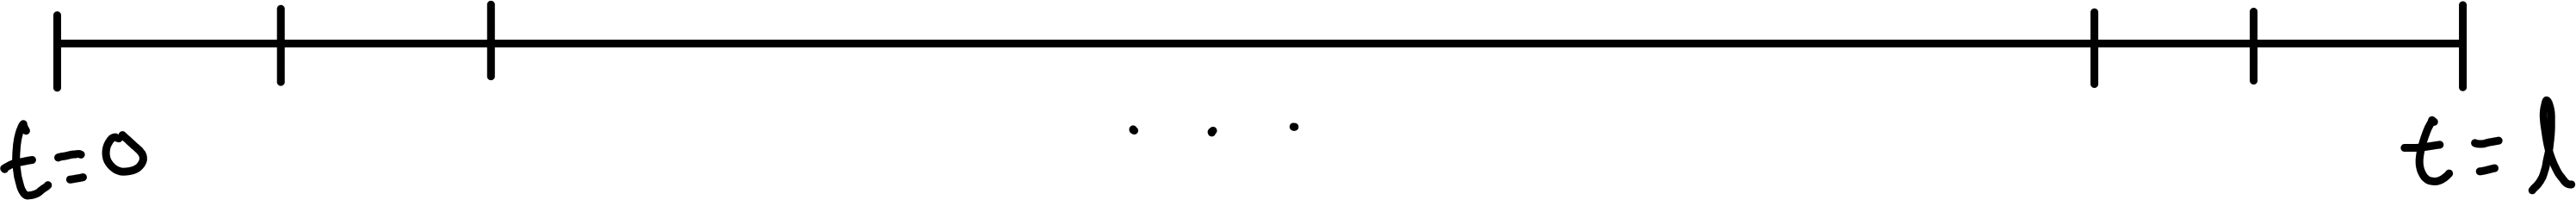
\includegraphics[height=5cm]{04-arrival} \par}
    \begin{itemize}
        \item Split time interval $[0, \lambda]$ into $n$ small intervals.
        \item Probability of an arrival in each interval is $p$, independently across intervals.
        \item Total no. of arrivals is $X_n$.
    \end{itemize} 

    \begin{align*}
        \mathbb{P}(X_n = k) &= \binom{n}{k} \left(\frac{\lambda}{n}\right)^k \left(1 - \frac{\lambda}{n}\right)^{n - k} \\
        \intertext{\color{blue} Fix $k$ and let $n \to \infty$}
        &= \frac{n!}{n^k (n - k)!} \times \underbracket{\frac{\lambda^k}{k!}}_{\text{no n}} \times \underbracket{\left(1 - \frac{\lambda}{n}\right)^n}_{\to e^{-\lambda}} \times \underbracket{\left(1 - \frac{1}{n}\right)^{-k}}_{\to 1} \\
        \frac{n!}{n^k (n - k)!} &= \frac{n (n-1) \dots (n - k + 1)}{n^k} \\
        &= 1 \times \left(1 - \frac{1}{n}\right) \times \left(1 - \frac{2}{n}\right) \times \dots \times \left(1 - \frac{k - 1}{n}\right) \\
        &\to 1 \quad \text{There are a fixed number of terms all converging to 1} \\
        \mathbb{P}(X_n = k) &\underset{n \to \infty}{\to} e^{-\lambda} \frac{\lambda^k}{k!}.
    \end{align*} 
    \color{blue} We might want to say $\operatorname{Bin}(n, \frac{\lambda}{n})$ converges to $\operatorname{Po}(\lambda)$, but what does convergence of random variables mean?
\end{example}

\subsection{Expectation}
$(\Omega, \mathcal{F}, \mathbb{P})$ and $X$ a discrete RV.
For now: $X$ only takes non-negative values. ``$X \geq 0$''

\begin{definition}[Expectation]
    The \vocab{expectation of $X$} (or \vocab{expected value} or \vocab{mean})
    \begin{align*}
        \mathbb{E}[X] &= \sum_{x \in \operatorname{Im}(X)} x \mathbb{P}(X = x) \\
        &= \sum_{\omega \in \Omega} X(\omega) \mathbb{P}(\{\omega\}) 
    \end{align*} 
    \color{blue} ``Average of values taken by $X$, weighted by $p_X$''.
\end{definition} 

\begin{example}[Uniform Dice]
    $X$ uniform on $\{1, 2, \dots, 6\}$
    \begin{align*}
        \mathbb{E}[X] &= \frac{1}{6} \cdot 1 + \frac{1}{6} \cdot 2 + \dots + \frac{1}{6} \cdot 6 \\
        &= 3.5 
    \end{align*} 
\end{example} 

\begin{note}
    $\mathbb{E}[X]$ need not be in $\operatorname{Im}(X)$.
\end{note}

\begin{example}[Binomial Distribution]
    Let $X \sim \operatorname{Binomial}(n, p)$
    \begin{align*}
        \mathbb{E}[X] &= \sum_{k=0}^{n} k \mathbb{P}(X = k) \\
        &= \sum_{k=0}^{n} k \binom{n}{k} p^k (1 - p)^k \\
        \color{blue} \emph{Trick:} \quad k \binom{n}{k} &\color{blue}=  \frac{k \times n!}{k! \times (n - k)!} \\
        &\color{blue}= \frac{n!}{(k - 1)! (n - k)!} \\
        &\color{blue}= n \binom{n - 1}{k - 1} \\
        \mathbb{E}[X] &= n \sum_{k=1}^{n} \binom{n - 1}{k - 1} p^k (1 - p)^k \\
        &= n p \sum_{k=1}^{n} \binom{n - 1}{k - 1} p^{k - 1} (1 - p)^k \\
        &= np \sum_{l=0}^{n - 1} \underbracket{\binom{n - 1}{l} p^l (1 - p)^{(n - 1) - l}}_{\color{blue} \text{pmf of } \operatorname{Bin}(n - 1, p)} \\
        &= np (p + (1 - p))^{n - 1} \\
        &= np.
    \end{align*} 
\end{example} 

\begin{note}
    We would like to say:
    \begin{align*}
        \mathbb{E}[\operatorname{Bin}(n, p)] &= \mathbb{E}[\operatorname{Bern}(p)] + \dots + \mathbb{E}[\operatorname{Bern}(p)]
    \end{align*} 
    We will be able to do this soon.
\end{note} 

\begin{example}[Poisson Distribution]
    Let $X \sim \operatorname{Poisson}(\lambda)$
    \begin{align*}
        \mathbb{E}[X] &= \sum_{k \geq 0} k \mathbb{P}(X = k) \\
        &= \sum_{k \geq 0} k \cdot e^{-\lambda} \frac{\lambda^k}{k!} \\
        &= \sum_{k \geq 1} e^{-\lambda} \frac{\lambda^k}{(k - 1)!} \\
        &= \lambda \sum_{k \geq 1} e^{-\lambda} \frac{\lambda^{k - 1}}{(k - 1)!} \quad \color{blue} \text{pmf of } \operatorname{Poisson}(\lambda) \\
        &= \lambda.
    \end{align*} 
\end{example} 

\begin{note}
    We would like to say
    \begin{align*}
        \mathbb{E}[\operatorname{Poisson}(\lambda)] \approx \mathbb{E}\left[\operatorname{Bin}\left(n, \frac{\lambda}{n}\right)\right] = \lambda
    \end{align*} 
    \color{blue} It is not true in general that $\mathbb{P}(X_n = k) \approx \mathbb{P}(X = k) \implies \mathbb{E}[X_n] \approx \mathbb{E}[X]$
\end{note} 

\begin{aside}{Not important}
    If $X$ can take on any real value (not necessarily $X \geq 0$)
    \begin{align*}
        \mathbb{E}[X] = \sum_{x \in \operatorname{Im}(X)} x \mathbb{P}(X = x)
    \end{align*} 
    unless: A, $\displaystyle \sum_{\substack{x > 0 \\ x \in \operatorname{Im}(X)}} x \mathbb{P}(X = x) = + \infty$ and B, $\displaystyle \sum_{\substack{x < 0 \\ x \in \operatorname{Im}(X)}} x \mathbb{P}(X = x) = - \infty$. \\
    Then we say $\mathbb{E}[X]$ is not defined.
    \color{red} Do we really want to study $\infty + \frac{2}{3} (- \infty)$ \color{black}
\end{aside} 

\underline{Summary}: 
\begin{itemize}
    \item A and B, $\mathbb{E}[X]$ is not defined.
    \item A but not B, $\mathbb{E}[X] = + \infty$.\footnote{Some people say not defined instead of letting $\mathbb{E}[X] =  \pm \infty$}
    \item B but not A, $\mathbb{E}[X] = - \infty$.
    \item neither A nor B, $X$ is then integrable i.e. $\mathbb{E}[X]$ absolutely converges.
\end{itemize} 

\begin{example}
    Most examples in the course are integrable \emph{except}: 
    \begin{itemize}
        \item $\mathbb{P}(X = n) = \frac{6}{\pi^2} \frac{1}{n^2}$ for $n \geq 1$.
        Note that $\sum \mathbb{P}(X = n) = 1$. \\
        Then $\mathbb{E}[X] = \sum \frac{6}{\pi^2} \frac{1}{n} = + \infty$.
        \item $\mathbb{P}(X = n) = \frac{3}{\pi^2} \frac{1}{n^2}$ for $n \in \mathbb{Z} \setminus \{0\}$.
        Then $\mathbb{E}[X]$ is not defined.
        \color{blue} ``It's symmetric so $\mathbb{E}[X] = 0$'', we have decided that this is wrong to prevent many things going wrong in second and third year courses in probability.
    \end{itemize} 
\end{example} 

\begin{example}[Indicator Function] \label{exm:exp-indi}
    $\mathbb{E}[1_A] = \mathbb{P}(A)$.
\end{example} 

\subsubsection{Properties of Expectation}

\begin{proposition} \label{prp:exp-1}
    If $X \geq 0$, then $\mathbb{E}[X] \geq 0$ with equality iff $\mathbb{P}(X = 0) = 1$. 
\end{proposition} 

\begin{proof}
    $\displaystyle \mathbb{E}[X] = \sum_{\substack{x \in \operatorname{Im}(X) \\ x \neq 0}} x \mathbb{P}(X = x)$
\end{proof} 

\begin{proposition}[Linearity of expectation] \label{prp:linear}
    Given random variables $X, Y$ (both integrable) on same probability space $\forall \; \lambda, \mu \in \mathbb{R}$
    \begin{align*}
        \mathbb{E}[\lambda X + \mu Y] &= \lambda \mathbb{E}[X] + \mu \mathbb{E}[Y] \\
        \text{Similarly} \quad \mathbb{E}[\lambda_1 X_1, + \dots + \lambda_n X_n] &= \lambda_1 \mathbb{E}[X_1] + \dots + \lambda_n \mathbb{E}[X_n]\footnote{holds for countably infinite collection though proof is omitted until more analysis experience.}
    \end{align*} 
\end{proposition} 

\begin{note}
    \emph{Independence} is \emph{NOT} a condition.
\end{note}  

\begin{proof}
    If $\Omega$ is countable:
    \begin{align*}
        \mathbb{E}[\lambda X + \mu Y] &= \Ccancel[blue]{\sum_{z \in \operatorname{Im}(\lambda X + \mu Y)} z \mathbb{P}(\lambda X + \mu Y = z)} \quad \color{blue} \text{awkward} \\
        &= \sum_{\omega \in \Omega} (\lambda X(\omega) + \mu Y(\omega)) \mathbb{P}(\{\omega\}) \\
        &= \lambda \sum_{\omega \in \Omega} X(\omega) \mathbb{P}(\{\omega\}) + \mu \sum_{\omega \in \Omega} Y(\omega) \mathbb{P}(\{\omega\}) \\
        &= \lambda \mathbb{E}[X] + \mu \mathbb{E}[Y].
    \end{align*} 
\end{proof} 

\begin{aside}{Aside - Special Cases}
    \begin{enumerate}
        \item If $\lambda, c \in \mathbb{R}$ then:
        \begin{enumerate}
            \item $\mathbb{E}[X + c] = \mathbb{E}[X] + c$
            \item $\mathbb{E}[\lambda X] = \lambda \mathbb{E}[X]$
        \end{enumerate} 
        \item \begin{enumerate}
            \item $X, Y$ random variables (both integrable) on same probability space.
            $\mathbb{E}[X + Y] = \mathbb{E}[X] + \mathbb{E}[Y]$.
            \item in fact $\lambda, \mu \in \mathbb{R}$ $\mathbb{E}[\lambda X + \mu Y] = \lambda \mathbb{E}[X] + \mu \mathbb{E}[Y]$ (similarly $\mathbb{E}[\lambda_1, X_1, + \dots + \lambda_n X_n] = \lambda_1 \mathbb{E}[X_1] + \dots + \lambda_n \mathbb{E}[X_n]$)
        \end{enumerate} 
    \end{enumerate} 
\end{aside} 

\begin{corollary}
    $X \geq Y$\footnote{$X(\omega) \geq Y(\omega) \quad \forall \; \omega \in \Omega$} then $\mathbb{E}[X] \geq \mathbb{E}[Y]$.
\end{corollary} 

\begin{proof}
    \begin{align*}
        X &= (X - Y) + Y \\
        \mathbb{E}[X] &= \mathbb{E}[X - Y] + \mathbb{E}[Y] \\
        X - Y \geq 0 &\implies \mathbb{E}[X - Y] \geq 0 \quad \text{by \Cref{prp:exp-1}}.
    \end{align*} 
\end{proof} 

\begin{example}[Counting Problems]
    $(\sigma(1), \dots, \sigma(n))$ uniform on $\Sigma_n$.
    $Z = |\{i : \sigma(i) = i\}| =$ number of fixed points.
    Let $A_i = \{\sigma(i) = i\}$, \color{blue} recall from \Cref{exm:indep1} $A_i$s \emph{not} independent. \color{black}

    \emph{Key step}:
    \begin{align*}
        Z &= 1_{A_1} + \dots + 1_{A_n} \\
        \mathbb{E}[Z] &= \mathbb{E}[1_{A_1} + \dots + 1_{A_n}] \\
        &= \mathbb{E}[1_{A_1}] + \dots + \mathbb{E}[1_{A_n}] \quad \text{by \nameref{prp:linear}} \\
        &= \mathbb{P}(A_1) + \dots + \mathbb{P}(A_n) \quad \text{by \Cref{exm:exp-indi}}\\
        &= \frac{1}{n} n = 1.
    \end{align*}
\end{example}

\begin{note}
    Same answer as $\operatorname{Bin}(n, \frac{1}{n})$
\end{note} 

\begin{proposition}
    If $X$ takes values in $\{0, 1, 2, \dots\}$ then
    \begin{align*}
        \mathbb{E}[X] = \sum_{k \geq 0} \mathbb{P}(X \geq k)
    \end{align*} 
\end{proposition} 

\begin{proof}
    One can carefully re-arrange the summands which is left as an exercise to the reader.
\end{proof} 

\begin{proof}[Alternative]
    Write $X = \sum_{k \geq 1} 1_{X \geq k}$\footnote{Sanity check: let $X = 7$, $1_{X \geq 1} = \dots = 1_{X \geq 7} = 1$ whilst $1_{X \geq 8} = 1_{X \geq 9} = \dots = 0$.} then take $\mathbb{E}[X]$:
    \begin{align*}
        \mathbb{E}[X] &= \mathbb{E}\left[\sum 1_{X \geq q}\right] \\
        &= \sum \mathbb{E}[1_{X \geq k}] \\
        &= \sum \mathbb{P}(X \geq k)
    \end{align*} 
\end{proof} 

\begin{claim}[Markov's Inequality] \label{clm:markov}
    Let $X \geq 0$ be a random variable.
    Then $\forall \; a > 0$:
    \begin{align*}
        \mathbb{P}(X \geq a) \leq \frac{\mathbb{E}[X]}{a}
    \end{align*} 
    \color{red} The LHS is interesting, e.g. if we want to bound the probability of an extreme outcome, whilst the RHS is easy to study.
\end{claim}

\begin{note} \color{blue}
    Is $a = \frac{\mathbb{E}[X]}{2}$ useful? No, we already know probabilities are less than 2. \\
    If $a$ is large it might be useful
\end{note} 

\begin{proof}
    Observe $X \geq a 1_{X \geq a}$\footnote{Check: If $X \in [0, a)$ then RHS $= 0$ else RHS $= a$.} and take $\mathbb{E}$
    \begin{align*}
        \mathbb{E}[X] &\geq a \mathbb{E}[1_{X \geq a}] \\
        &= a \mathbb{P}(X \geq a)
    \end{align*} 
\end{proof} 

\begin{note} \color{red}
    Markov's Inequality is also true for continuous RVs.
\end{note} 

\subsubsection{Studying $\mathbb{E}[f(X)]$}
Let $f: \mathbb{R} \to \mathbb{R}$ be a function.
Then $f(X)$ is also a \emph{random variable}\footnote{\color{blue} $X: \Omega \to \mathbb{R}$ so $f(X) : \Omega \to \mathbb{R}$.}.

\begin{claim} ~\vspace*{-1.5\baselineskip}
    \begin{align*}
        \mathbb{E}[f(X)] &= \sum_{x \in \operatorname{Im}(X)} f(x) \mathbb{P}(X = x)\footnote{if it exists}.
    \end{align*} 
\end{claim} 

\begin{proof}
    Let $A = \operatorname{Im}(f(x)) = \{f(x) : x \in \operatorname{Im}(X)\}$.
    Starting with RHS
    \begin{align*}
        \sum_{x \in \operatorname{Im}(X)} f(x) \mathbb{P}(X = x) &= \sum_{y \in A} \sum_{\substack{x \in \operatorname{Im}(X) \\ f(x) = y}} f(x) \mathbb{P}(X = x) \\
        &= \sum_{y \in A} y \sum_{\substack{x \in \operatorname{Im}(X) \\ f(x) = y}} \mathbb{P}(X = x) \\
        &= \sum_{y \in A} y \mathbb{P}(f(X) = y) \quad \text{by additivity} \\
        &= \mathbb{E}[f(X)]
    \end{align*}  
\end{proof}

\subsection{Variance}
\underline{Motivation}
\begin{align*}
    U_n &\sim \operatorname{Uniform}(\{-n, -n + 1, \dots, n\}) \\
    V_n &\sim \operatorname{Uniform}(\{-n, n\}) \\
    Z_n &= 0 \\
    S_n &= \text{random walk for $n$ steps} \\
    &\sim n - 2 \operatorname{Bin}\left( n, \frac{1}{2} \right)
\end{align*} 
All of these have \emph{$\mathbb{E} = 0$}.

\color{blue} Variance is a way to ``measure how concentrated a RV is around its mean''. \color{black}

\begin{definition}
    The \vocab{variance} of $X$ is:
    \begin{align*}
        \Var(X) &= \mathbb{E}\left[(X - \mathbb{E}[X])^2 \right]
    \end{align*} 
\end{definition} 

\begin{proposition}
    $\Var(X) \geq 0$ with equality $\iff \mathbb{P}(X = \mathbb{E}[X]) = 1$ (as $(X - \mathbb{E}[X])^2$ so by \Cref{prp:exp-1}).
\end{proposition} 

\begin{definition}[Alternative characterisation] ~\vspace*{-1.5\baselineskip}
    \begin{align*}
        \Var(X) &= \mathbb{E}\left[X^2\right] - \left( \mathbb{E}[X] \right)^2 \quad (\geq 0)
    \end{align*} 
\end{definition} 

\begin{proof}
    Write $\mu = \mathbb{E}[X]$
    \begin{align*}
        \Var(X) &= \mathbb{E}\left[ (X - \mu)^2 \right] \\
        &= \mathbb{E}\left[X^2 - 2\mu X + \mu^2\right] \\
        &= \mathbb{E}[X^2] - 2 \mu \underbracket{\mathbb{E}[X]}_\mu + \mu^2 \\
        &= \mathbb{E}[X^2] - \mu^2
    \end{align*} 
\end{proof} 

\begin{proposition}[Properties]
    If $\lambda, c \in \mathbb{R}$
    \begin{itemize}
        \item $\Var(\lambda X) = \lambda^2 \Var(X)$.
        \item $\Var(X + c) = \Var(X)$
    \end{itemize} 
\end{proposition} 

\begin{proof}
    \begin{align*}
        \mathbb{E}[X + c] &= \mu + c \\
        \Var(X + c) &= \mathbb{E}\left[\left( X + c - (\mu + c)^2 \right)\right] \\
        &= \mathbb{E}\left[(X - \mu)^2\right] \\
        &= \Var(X).
    \end{align*} 
\end{proof} 

\begin{example}[Poisson Distribution]
    Let $X \sim \operatorname{Poisson}(\lambda)$
    \begin{align*}
        \Var(X) &= \mathbb{E}[X^2] - \lambda^2 \\
        \intertext{\color{blue} ``Falling factorial trick'': sometimes easier to calculate $\mathbb{E}[X (X - 1)]$ than $\mathbb{E}[X^2]$}
        \mathbb{E}[X(X-1)] &= \sum_{k \geq 2} \underbracket{k(k-1)}_{\color{blue} \text{function}} \underbracket{e^{- \lambda} \frac{\lambda^k}{k!}}_{\color{blue} \text{PMF}} \\
        &= \lambda^2 e^{- \lambda} \underbracket{\sum_{k \geq 2} \frac{\lambda^{k - 1}}{(k - 2)!}}_{e^\lambda} \\
        &= \lambda^2 \\
        \mathbb{E}[X^2] &= \mathbb{E}[X (X - 1)] + \mathbb{E}[X] \\
        &= \lambda^2 + \lambda \\
        \Var(X) &= \lambda
    \end{align*} 
\end{example} 

\begin{example}[Geometric Distribution]
    Let $Y \sim \operatorname{Geom}(p)$ where $Y \in \mathbb{N}$.
    \begin{align*}
        \mathbb{E}[Y] &= \frac{1}{p},\ \Var(Y) = \frac{1 - p}{p^2}.
    \end{align*} 
    Proof left as an exercise.
\end{example} 

\color{blue}
\begin{note}
    $\lambda$ large: $\Var(x) = \mathbb{E}[X]$, \color{red}more concentrated \color{blue} \\
    $p$ small: $\Var(Y) \approx \frac{1}{p^2} = \left( \mathbb{E}[X] \right)^2$.
\end{note} 

\begin{example}[Bernouli Distribution]
    Let $X \sim \operatorname{Bern}(p)$.
    \begin{align*}
        \mathbb{E}[X] &= 1 \times p = p \\
        \mathbb{E}[X^2] &= 1^2 \times p = p \\
        \Var(X) &= p - p^2 \\
        &= p(1-p)
    \end{align*} 
\end{example} 

\begin{example}[Binomial Distribution] \label{exm:var-bin}
    Let $X \sim \operatorname{Bin}(n, p)$
    \begin{align*}
        \mathbb{E}[X] &= np  \\
        \mathbb{E}\left[X^2\right] &= \color{red} \text{ugly}
    \end{align*} 
\end{example} 

\subsubsection{Sums of RVs}

\color{blue} \underline{Goal}: Study $\Var(X_1 + \dots + X_n)$. Do the $X_i$s need to be independent. \color{black}

\begin{proposition}[Preliminary: Expectation of Product of RVs] \label{prp:expprod}
    If $X, Y$ are \color{red} independent \color{black} RVs and $f, g$ are functions $\mathbb{R} \to \mathbb{R}$. \\
    Then: $\mathbb{E}[f(X) g(Y)] = \mathbb{E}[f(X)] \mathbb{E}[g(Y)]$ \color{blue} ``Splits as a product'' \color{black}.
\end{proposition} 

\begin{example}
    $\mathbb{E}[XY] = \mathbb{E}[X] \mathbb{E}[Y]$
\end{example} 

\begin{example}
    Let $f(x) = g(x) = z^x$ (or $e^{tx}$).
\end{example} 

\begin{proof}
    \color{blue} (X, Y discrete) \color{black}
    \begin{align*}
        \text{LHS} &= \sum_{x, y \in \operatorname{Im}} f(x) g(y) \mathbb{P}(X = x, Y = y) \\
        &= \sum_{x, y \in \operatorname{Im}} f(x) g(y) \mathbb{P}(X = x) \mathbb{P}(Y = y) \\
        &= \left[\sum_{x \in \operatorname{Im}} f(x) \mathbb{P}(X = x) \right] \left[\sum_{y \in \operatorname{Im}} g(x) \mathbb{P}(Y = y) \right] \\
        &= \mathbb{E}[f(X)] \mathbb{E}[g(Y)]
    \end{align*} 
\end{proof} 

\begin{proposition}[Sums of independent RVs]
    Let $X_1, \dots, X_n$ be \underline{independent}.
    Then
    \begin{align*}
        \Var(X_1 + \dots + X_n) = \Var(X_1) + \dots + \Var(X_n)
    \end{align*} 
\end{proposition} 

\begin{proof}
    (Suffices to Prove (STP) $n = 2$). 
    Say $\mathbb{E}[X] = \mu,\, \mathbb{E}[Y] = \nu$
    \begin{align*}
        \Var(X + Y) &= \mathbb{E}\left[ \left( X + Y - \mu - \nu \right)^2 \right] \\
        &= \mathbb{E} \left[ \left( X - \mu \right)^2 \right] + \mathbb{E}\left[ (Y - \nu)^2 \right] + 2 \mathbb{E}[(X - \mu)(Y - \nu)]. \\
        &= \Var(X) + \Var(Y) + 2 \mathbb{E}[X - \mu] \mathbb{E}[Y - \nu] \\
        &= \Var(X) + \Var(Y).
    \end{align*} 
\end{proof} 


\begin{example}[Binomial]
    Going back to \nameref{exm:var-bin}, $\Var(\operatorname{Bin}(n, p)) = n p(1-p)$.
\end{example} 

\underline{Goal}: Study $\Var(X + Y)$ when $X, Y$ not independent.

\begin{definition}[Covariance]
    Let $X, Y$ be two RVs.
    Their \vocab{covariance} is 
    \begin{align*}
        \Cov(X, Y) &= \mathbb{E}\left[ (X - \mathbb{E}[X]) (Y - \mathbb{E}[Y]) \right]
    \end{align*} 
    \color{blue} ``Measures how dependent $X, Y$ are and in which \underline{direction}'' ($X$ large $\implies Y$ larger if $\Cov > 0$ else $Y$ smaller).
\end{definition} 

\begin{proposition}[Properties] ~\vspace*{-1.5\baselineskip}
    \begin{align*}
        \Cov(X, Y) &= \Cov(Y, X) \\
        \Cov(X, X) &= \Var(X)
    \end{align*} 
\end{proposition} 

\begin{definition}[Alternative Characterisation] ~\vspace*{-1.5\baselineskip}
    \begin{align*}
        \Cov(X, Y) &= \mathbb{E}[XY] - \mathbb{E}[X]\mathbb{E}[Y]
    \end{align*} 
\end{definition} 

\begin{proof}
    \begin{align*}
        \Cov(X, Y) &= \mathbb{E}\left[ (X- \mu) (Y - \nu) \right] \\
        &= \mathbb{E}[XY] - \mu \underbracket{\mathbb{E}[Y]}_\nu - \nu \underbracket{\mathbb{E}[X]}_\mu + \mu \nu \\
        &= \mathbb{E}[XY] - \mu \nu.
    \end{align*} 
\end{proof} 

\begin{proposition}[More Properties]
    Let $\lambda \in \mathbb{R}$
    \begin{align*}
        \Cov(\lambda, X) &= 0 \\
        \Cov(X + \lambda, Y) &= \Cov(X, Y) \\
        \Cov(\lambda X, Y) &= \lambda \Cov(X, Y) \\
        \Var(X + Y) &= \Var(X) + \Var(Y) + 2 \Cov(X, Y)
    \end{align*} 
\end{proposition} 

\color{blue}
Covariance is \underline{linear} in each argument i.e. $\Cov(\sum \lambda_i X_i, Y) = \sum \lambda_i \Cov(X_i, Y)$ and $\Cov (\sum \lambda_i X_i, \sum \mu_j Y_j)= \sum_{i=1}^{n} \sum_{j=1}^{m} \lambda_i \mu_j \Cov(X_i, Y_j)$.
\color{black}

\begin{proposition}[Sums of RVs] ~\vspace*{-1.5\baselineskip}
    \begin{align*}
        \Var\left( \sum_{i=1}^{n} X_i \right) &= \Cov\left( \sum_{i=1}^{n} X_i, \sum_{i=1}^{n} X_i \right) \\
        &= \sum_{i=1}^{n} \Var(X_i) + \sum_{i \neq j} \Cov(X_i, X_j)\footnote{or $2 \sum_{i < j} \Cov(X_i, X_j)$}
    \end{align*} 
\end{proposition} 

\begin{proposition}
    $X, Y$ independent $\implies \Cov(X, Y) = 0$, \color{red} the converse is false.
\end{proposition} 

\begin{example}
    Let $Y = - X$, $\Var(Y) = \Var(X)$. 
    So $\Var(X + Y) = \Var(0) = 0 \neq \Var(X) + \Var(Y)$.
\end{example} 

\begin{example}[Uniform Permutation]
    Let $(\sigma(1), \dots, \sigma(n))$ be uniformly chosen on $\Sigma_n$.
    Let $A_i = \{\sigma(i) = i\}$ and $N = 1_{A_1} + \dots + 1_{A_n}$ ($N$ is the number of fixed points). \\
    \begin{align*}
        \mathbb{E}[N] &= n \times \frac{1}{n} = 1
        \intertext{$A_i$ and $A_j$ are \emph{not} independent}
        \Var(1_{A_1}) &= \frac{1}{n} \left( 1 - \frac{1}{n} \right) \\
        \Cov(1_{A_i}, 1_{A_j}) &= \mathbb{E}[1_{A_i} 1_{A_j}] - \mathbb{E}[1_{A_i}] \mathbb{E}[1_{A_j}] \\
        &= \mathbb{E}[1_{A_i \cap A_j}] - \mathbb{E}[1_{A_i}] \mathbb{E}[1_{A_j}] \\
        &= \mathbb{P}(A_i \cap A_j) - \mathbb{P}(A_i) \mathbb{P}(A_j) \\
        &= \frac{1}{n (n - 1)} - \frac{1}{n} \times \frac{1}{n} \\
        &= \frac{1}{n^2 (n - 1)} > 0
        \intertext{\color{blue} Note: $\Cov$ doesn't depend on $i, j$}
        \Var(N) &= \sum_{i=1}^{n} \Var(1_{A_i}) + \sum_{i \neq j} \Cov(1_{A_i}, 1_{A_j}) \\
        &= n \times n \left( 1 - \frac{1}{n} \right) + n(n-1) \times \frac{1}{n^2 (n - 1)} \\
        &= 1 - \frac{1}{n} + \frac{1}{n} \\
        &= 1.
    \end{align*}
    \emph{Compare} with $\operatorname{Bin}\left( n, \frac{1}{n} \right)$:
    $\mathbb{E} = 1$, $\Var = n \times \frac{1}{n} \left( 1 - \frac{1}{n} \right) = 1 - \frac{1}{n}$.
\end{example} 

\subsubsection{Chebyshev's Inequality}

\begin{proposition}[Chebyshev's Inequality] \label{prp:cheby}
    Let $X$ be a RV, $\mathbb{E}[X] = \mu$ finite, $\Var(X) = \sigma^2 < \infty$.
    \begin{align*}
        \mathbb{P}(|X - \mu| \geq \lambda) \leq \frac{\Var(X)}{\lambda^2}
    \end{align*} 
    \color{blue} Remember the proof, not the statement.
\end{proposition} 

\begin{proof}
    \underline{Idea}: Apply \nameref{clm:markov} to $(X - \mu)^2$.
    \begin{align*}
        \mathbb{P}\left( (X - \mu)^2 \geq \lambda^2 \right) &\leq \frac{\mathbb{E}\left[ (X - \mu)^2 \right]}{\lambda^2} \\
        &= \frac{\Var(X)}{\lambda^2}
    \end{align*} 
\end{proof} 

\color{red} \underline{Danger}: Applying \nameref{clm:markov} to $|X - \mu|$, $\mathbb{E}\left[|X - \mu|\right]$ is less nice than $\mathbb{E}\left[ (X - \mu)^2 \right]$. \color{black}

\underline{Comments}
\begin{itemize}
    \item Chebyshev's Inequality gives better bounds than Markov's Inequality (decays with $\lambda^2$ instead of $\lambda$).
    \item We can apply it to all RVs, not just those $\geq 0$.
    \item Caveat: We need $\Var(X) < \infty$ which is a stronger condition than $\mathbb{E}[X] < \infty$.
\end{itemize} 

\begin{definition}[Standard Deviation]
    $\sqrt{\Var(X)}$ is the \vocab{standard deviation}, $\sigma$, of $X$.
\end{definition} 
It has the same ``units'' as $X$ but not many nice properties so $\Var$ is generally preferred.

We can rewrite Chebyshev as $\mathbb{P}(|X - \mu| \geq k \sigma) \leq 1 / k^2$

\subsection{Conditional Expectation}
\underline{Setting}: $(\Omega, \mathcal{F}, \mathbb{P})$. \\
Recall the definition of \nameref{def:condition}. 

\begin{definition}[Conditional Expectation]
    $B \in \mathcal{F}$ with $\mathbb{P}(B) > 0$, $X$ a RV.
    The \vocab{conditional expectation} is 
    \begin{align*}
        \mathbb{E}[X \mid B] &= \frac{\mathbb{E}[X 1_{B}]}{\mathbb{P}(B)}
    \end{align*} 
\end{definition} 

\begin{example}[Uniform Dice]
    Let $X$ be a dice, uniform on $\{1, \dots, 6\}$.
    \begin{align*}
        \mathbb{E}[X \mid X \text{ prime}] &= \frac{\frac{1}{6} [0 + 2 + 3 + 0 + 5 + 0]}{\frac{1}{2}} \\
        &= \frac{1}{3} (2 + 3 + 5) \\
        &= \frac{10}{3}.
    \end{align*} 
\end{example} 

\begin{definition}[Alternative Characterisation] ~\vspace*{-1.5\baselineskip}
    \begin{align*}
        \mathbb{E}[X \mid B] &= \sum_{x \in \operatorname{Im} X} x \mathbb{P}(X = x \mid B).
    \end{align*} 
\end{definition} 

\begin{proof}
    \begin{align*}
        \text{RHS } &= \sum \frac{x \mathbb{P}(\{X = x\} \cap B)}{\mathbb{P}(B)} \\
        &= \sum_{\substack{x \neq 0 \\ x \in \operatorname{Im} X}} \frac{x \mathbb{P}(X 1_B = x)}{\mathbb{P}(B)} \\
        \text{Note: } \mathbb{E}[X 1_B] &= \sum_{\substack{x \neq 0 \\ x \in \operatorname{Im} X}} x \mathbb{P}(X 1_B = x)
    \end{align*} 
\end{proof} 

\begin{proposition}[Law of Total Expectation] \label{prp:lte}
    Let $(B_1, B_2, \dots)$ be a finite or countably-infinite partition of $\Omega$ with $B_n \in \mathcal{F} \quad \forall \; n$ s.t. $\mathbb{P}(B_n) > 0$.
    $X$ a RV.
    \begin{align*}
        \mathbb{E}[X] &= \sum_n \mathbb{E}[X \mid B_n] \mathbb{P}(B_n).
    \end{align*} 
\end{proposition} 

\begin{example}
    Let $X = 1_A$ we recover the \nameref{thm:ltp}.
\end{example} 

\begin{proof}
    \begin{align*}
        \text{RHS } &= \sum_n \mathbb{E}[X 1_{B_n}] \\
        &= \mathbb{E}\left[X \cdot (1_{B_1} + \dots + 1_{B_n}) \right] \quad \text{by \nameref{prp:linear}}\\
        &= \mathbb{E}[X \cdot 1] \\
        &= \mathbb{E}[X].
    \end{align*} 
\end{proof} 

\underline{Application}: Two stage randomness where $(B_n)$ describes what happens in stage 1.

\begin{example}[Sums of random number of terms]
    Let $(X_n)_{n \geq 1}$ be IID and $N \in \{0, 1, 2, \dots\}$ be a random index independent of $(X_n)$.
    $S_n = X_1 + \dots + X_n$ with $\mathbb{E}[X_n] = \mu$ so $\mathbb{E}[S_n] = n \mu$.
    Then
    \begin{align*}
        \mathbb{E}[S_N] &= \sum_{n \geq 0} \mathbb{E}[S_N \mid N = n] \mathbb{P}(N = n) \\
        &= \sum \mathbb{E}[S_{\color{red} n}] \mathbb{P}(N = n)\footnote{KEY STEP $\mathbb{E}[S_N \mid N = n] = \mathbb{E}[S_n \mid N = n] = \mathbb{E}[S_n]$ last step follows as $S_n$ and $\{N = n\}$ are independent.} \\
        &= \sum_{n \geq 0} n \mu \mathbb{P}(N = n) \\
        &= \mu \mathbb{E}[N].
    \end{align*}
\end{example} 

\subsection{Random Walks}

\begin{definition}[Random Walk]
    Let $(X_n)_{n \geq 1}$ be IID RVs then $S_n = x_0 + X_1 + \dots + X_n$. $(S_0, S_1, S_2, \dots)$ is a random process called a \vocab{Random Walk} started from $x_0$.
\end{definition} 

\subsubsection{Simple Random Walk (SRW) on $\mathbb{Z}$ - Main example in our course}

\begin{definition}[Simple Random Walk]
    A \vocab{simple random walk} has $P(X_i = + 1) = p$ and $\mathbb{P}(X = - 1) = q = 1-p$.
    $x_0 \in \mathbb{Z}$ and is often $0$. \\
    It is ``symmetric'' in the \underline{special case} where $p = q = \frac{1}{2}$.
\end{definition} 

\begin{example}
    $\mathbb{P}(S_2 = x_0) = pq + qp = 2pq$
\end{example} 

\underline{Useful interpretation}: A gamble repeatedly plays a game where he wins $\pounds 1$ with $\mathbb{P} = p$, loses $\pounds 1$ with $\mathbb{P} = q$. \\
Often: stops at $\pounds 0$.

\begin{question}
    Suppose the gambler starts with $\pounds x$ at time $0$.
    What is the probability he reaches $\pounds a$ before $\pounds 0$. ($0 < x < a$)
\end{question} 

\begin{figure}[h] 
    \centering 
    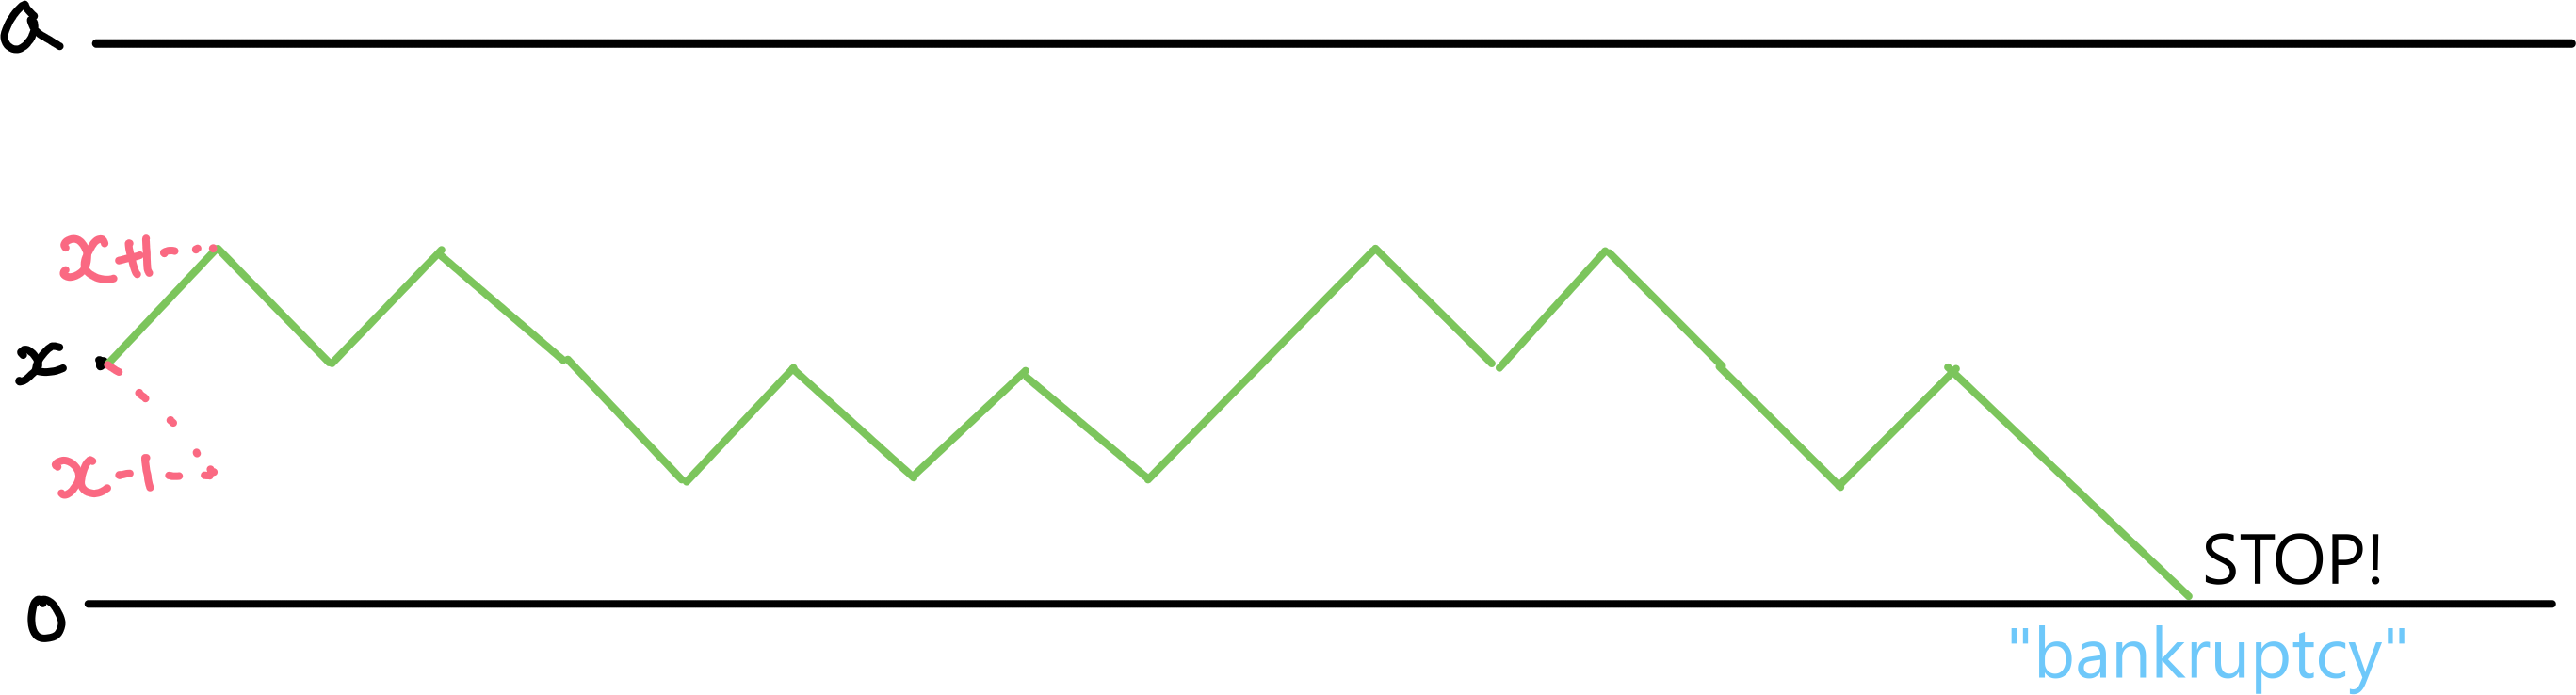
\includegraphics[height=5cm]{04-ruin} 
\end{figure}

\begin{notation}
    $\mathbb{P}_x(\cdot) = \mathbb{P}(\cdot \mid x_0 = x)$ \color{blue} ``measure of RW started from $x_0$.''
\end{notation} 

\begin{answer}
    \underline{Key idea}: Conditional on $S_1 = z$, $(S_1, S_2, \dots)$ is a random walk started from $z$. \\
    Apply \nameref{thm:ltp}
    \begin{align*}
        \mathbb{P}_x(S \text{ hits a before 0}) &= \sum\footnote{Subscript: $z \in \operatorname{Im}(S_1)$ but we will not bother with that any more} \overbracket{\mathbb{P}_x(S \text{ hits a before 0} \mid S_1 = z)}^{\color{red} \text{Interpret this.} \color{black}} \mathbb{P}_x(S_1 = z) \\
        &= \sum_z \mathbb{P}_z (S \text{ hits a before 0}) \mathbb{P}_x(S_1 = z) \\
        \text{let } h_x &= \mathbb{P}_x(S \text{ hits a before 0}). \\
        S_1 &= x \pm 1 \\
        h_x &= p h_{x + 1} + q h_{x - 1}.
    \end{align*} 
    Important to specify boundary conditions: $h_0 = 0$, $h_a = 1$

    \underline{Solving Linear Recurrence Equations} \\
    $p h_{x + 1} - h_x + q h_{x - 1} = 0$ is a homogenous equation whose solutions form a vector space.
    We want to find two LI solutions and we guess $h_x = \lambda^x$
    So \begin{align*}
        p \lambda^{x + 1} - \lambda^x + q \lambda^{x - 1} &= 0 \\
        p \lambda^2 - \lambda + q &= 0 \\
        \lambda &= 1, \frac{q}{p}
    \intertext{\underline{Case $q \neq p$}}
        h_x &= A + B \left( \frac{q}{p} \right)^x \\
        \intertext{Use BCs to find A,B: }
        x = 0 : h_0 &= 0 = A + B \\
        x = a : h_a &= 1 = A + B\left( \frac{q}{p} \right)^a \\
        h_x &= \frac{\left( \frac{q}{p} \right)^x - 1}{\left( \frac{q}{p} \right)^a - 1}.
    \end{align*} 
    
    \underline{Case $p = q = \frac{1}{2}$:} \\
    Note $h_x = x$ \color{blue}, ``$x$ is the average of $x + 1$ and $x - 1$''. \color{black} \\
    General solution: $h_x = A + Bx$
    \begin{align*}
        h_0 &= 0 = A \\
        h_a &= 1 = Ba \\
        h_x &= \frac{x}{a}
    \end{align*} 
\end{answer} 

\color{blue}
Probability sanity check: $p = q = \frac{1}{2}$. ``Fair game'' \\
Study: Expected profit if you start from $\pounds x$ and play until time $T$.
\begin{align*}
    \mathbb{E}_x[S_T] &= a \mathbb{P}_x(S_T = a) + 0 \times \mathbb{P}_x(S_T = 0) \\
    &= a h_x = x
\end{align*} 
Fits our intuition for fair games. \checkmark
\color{black}

\begin{question}
    Suppose the gambler starts with $\pounds x$ at time $0$.
    What is the expected absorption time, $T = \min \{ n \geq 0 : S_n = 0 \text{ or } S_n = a\}$. \color{blue} ``first time $S$ hits $\{0, a\}$'' \color{black}
\end{question} 

\begin{answer}
    Apply \nameref{prp:lte}\\
    We want $\mathbb{E}_x[T]$ ($\mathbb{E}[T]$ when we start from $x$) which we label as $\tau_x$
    \begin{align*}
        \tau_x &= \mathbb{E}_x[T] \\
        &= p \overbracket{\mathbb{E}_x[T \mid S_1 = x + 1]}^{\color{red} \text{Interpret this.} \color{black}}\footnote{\color{blue} ``As if we started from $(x + 1)$ and incremented time by one unit.''} + q \mathbb{E}_x[T \mid S_1 = x - 1] \\
        &= p \mathbb{E}_{x + 1}[T + 1] + q \mathbb{E}_{x - 1}[T - 1] \\
        &= p (1 + \mathbb{E}_{x + 1}[T]) + q(1 + \mathbb{E}_{x - 1}[T]) \\
        &= 1 + p \tau_{x + 1} + q \tau_{x - 1}
    \end{align*} 
    Boundary conditions: $\tau_0 = \tau_a = 0$ \color{blue} ``We're already there'' \color{black}.

    We already solved the homogenous case of this equation previously. 
    We want to find a \emph{particular solution}, \color{blue} guess: ``one level more complicated than general solution'' \color{black}

    \underline{$p \neq q$}: Guess: $\tau_x = \frac{x}{q - p}$ works as a particular solution

    \underline{$p = q = \frac{1}{2}$}: Guess $\tau_x = C x^2$ \emph{might} work
    \begin{gather*}
        \text{Sub in:} \ \frac{C}{2} (x + 1)^2 - C x^2 + \frac{C}{2} (x - 1)^2 = - 1 \\
        C = -1 \\
        \tau_x = A + Bx - x^2 \\
        \tau_0 = \tau_a = 0 \text{ and } \tau_x \geq 0\\
        \therefore \tau_x = x (a - x) 
    \end{gather*} 
\end{answer} 

\subsubsection{Unbounded RW: ``Gambler's Ruin'}

\begin{figure}[h] 
    \centering 
    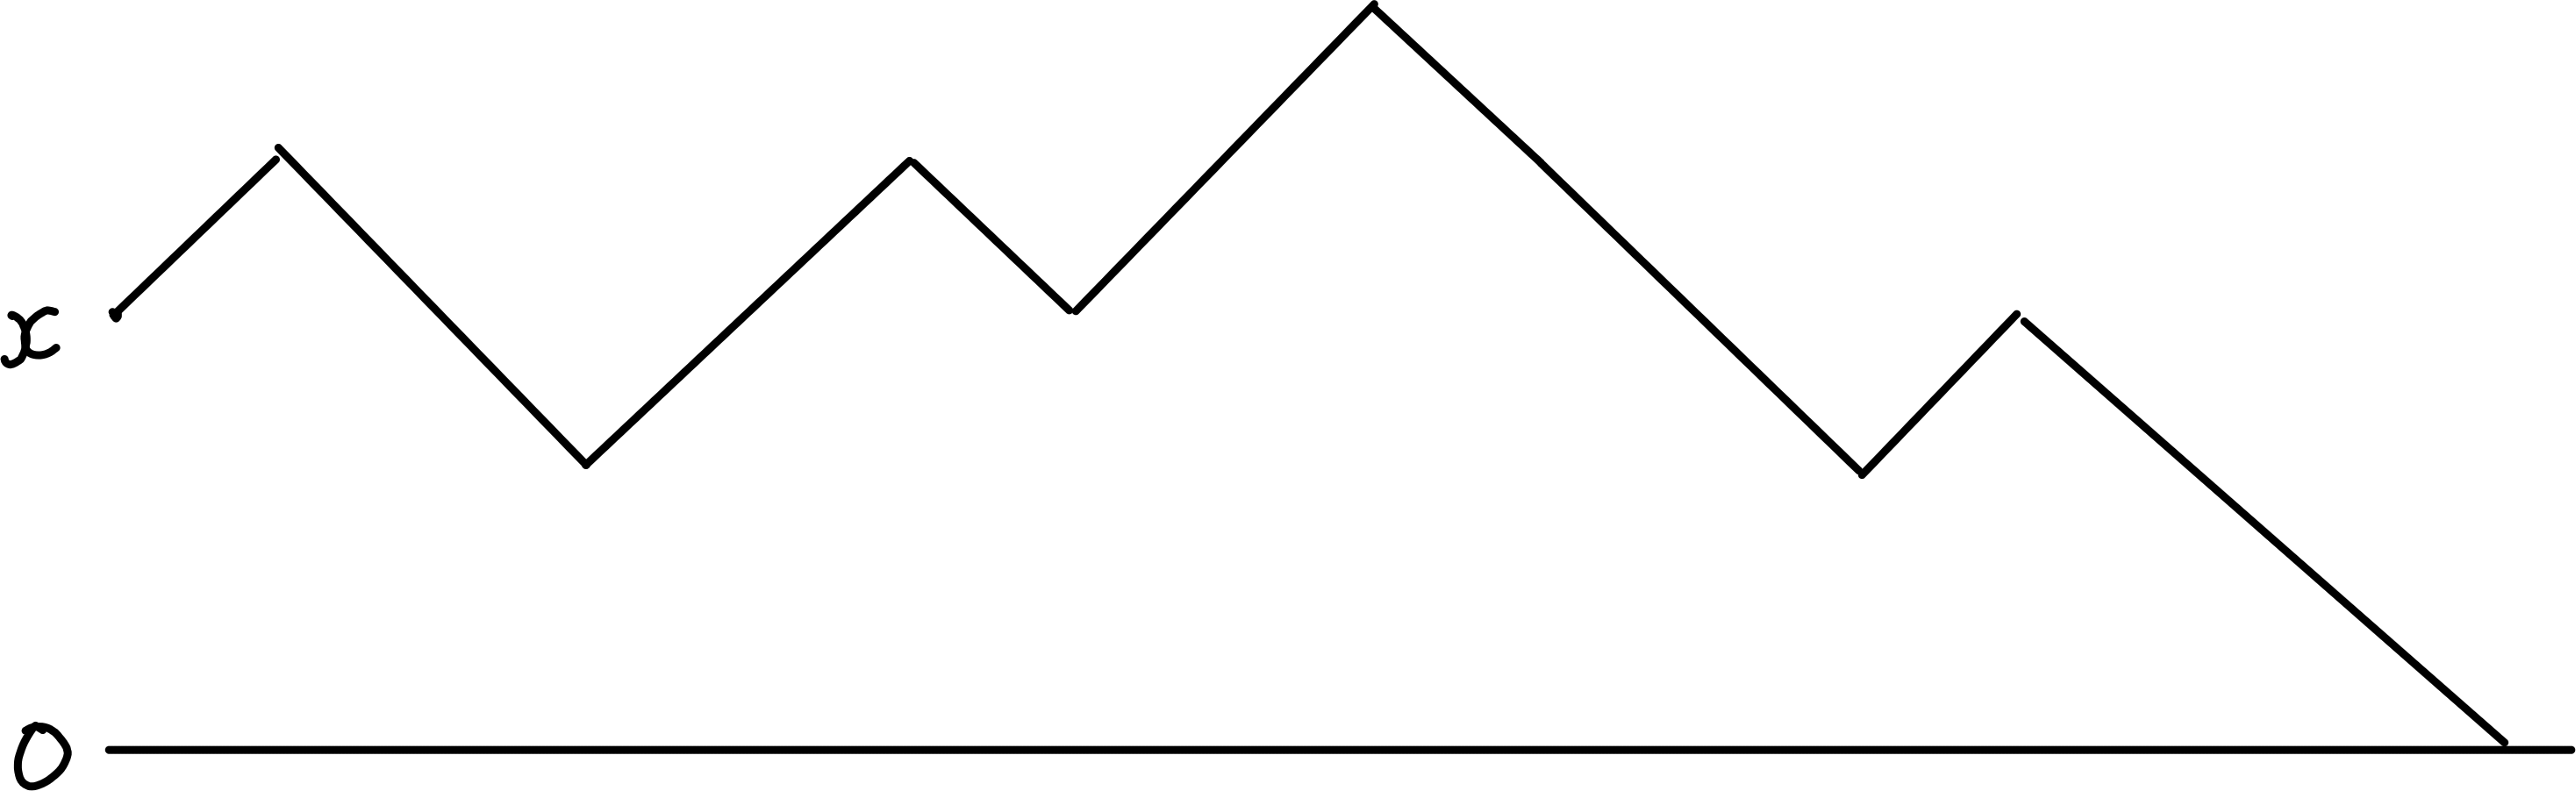
\includegraphics[height=5cm]{04-gamblers} 
\end{figure}

\begin{align*}
    \mathbb{P}_x(\text{hit } 0) &= \lim_{a \to \infty} \mathbb{P}_x(\text{hit $0$ before $a$}) \\
    &= \lim_{a \to \infty} 1 - h_x \\
    &= \begin{cases}
        (\frac{q}{p})^x & p > q \\
        1 & p \leq q
    \end{cases} \\
    \text{When $p = \frac{1}{2}$:} \quad \mathbb{E}_x[\text{time to hit } 0] &\geq \mathbb{E}_x[\text{time to hit $0$ or $a$}] \\
    &= x(a-x) \to \infty \text{ as } a \to \infty
\end{align*} 

\underline{Key conclusion}: $T_x$ (time to hit $0$ from $x$) is for $p = \frac{1}{2}$ finite with probability $1$ and has infinite expectation.

\begin{aside}{Comment (non - examinable)}
    Alternative derivation of $\mathbb{E}[T_1] = \infty$. \\
    $\mathbb{E}[T_2] = 2 \mathbb{E}[T_1]$ as going from $2 \to 1$ is the same as going from $1 \to 0$.
    \begin{align*}
        \mathbb{E}[T_1] &= \frac{1}{2} \times 1 + \frac{1}{2} \left( 1 + \mathbb{E}[T_2] \right) \\
        &= 1 + \mathbb{E}[T_1]
    \end{align*} 
    We conclude that $\mathbb{E}[T_1] = \infty$. \\
\end{aside} 

\subsection{Generating Functions}

\begin{definition}[Probability Generating Function]
    Let $X$ be a RV taking values in $\{0, 1, 2, \dots\}$. The \vocab{probability generating function} of $X$ is 
    \begin{align*}
        G_X(z) &= \mathbb{E}\left[ z^X \right] = \sum_{k \geq 0} z^k \mathbb{P}(X = k). 
    \end{align*} 
    Analytic comment: $G_X : (-1, 1) \to \mathbb{R}$.
\end{definition} 

\underline{Idea}: ``A pgf \emph{encodes} the distribution of $X$ as a function with nice analytic properties.''

\begin{example}[Bernoulli]
    Let $X \sim \operatorname{Bern}(p)$
    \begin{align*}
        G_X(z) &= z^0 \mathbb{P}(X = 0) + z \mathbb{P}(X = 1) \\
        &= (1-p) + pz.
    \end{align*} 
\end{example} 

\begin{example}[Poisson]
    Let $X \sim \operatorname{Poi}(\lambda)$
    \begin{align*}
        G_X(z) &= \sum_{k \geq 0} z^k e^{- \lambda} \frac{\lambda^k}{k!} \\
        &= e^{- \lambda} \sum_{k \geq 0} \frac{(\lambda z)^k}{k!} \\
        &= e^{- \lambda} e^{\lambda z} \\
        &= e^{\lambda (z - 1)}
    \end{align*} 
\end{example} 

\begin{note}
    $G_X(0) = 0^0 \mathbb{P}(X = 0) = \mathbb{P}(X = 0)$.
\end{note} 

\begin{proposition}[Recovering PMF from PGF]
    $\mathbb{P}(X = n) = \frac{1}{n!} G_X^{(n)} (0)$
\end{proposition} 

\begin{proof}
    \underline{Idea}: Differentiate $n$ times
    \begin{align*}
        \frac{d^n}{d z^n} G_X(z) &= \sum_{k \geq 0} \frac{d^n}{d z^n} (z^k) \mathbb{P}(X = k) \\
        &= \sum_{k \geq 0} \frac{k!}{(k - n)!} z^{k - n} \mathbb{P}(X = k) \\
        &= \sum_{k \geq n} \frac{k!}{(k - n)!} z^{k - n} \mathbb{P}(X = k) \\
        &= \sum_{l \geq 0} \frac{(l + n)!}{l!} z^l \mathbb{P}(X = l + n) \\
        \frac{d^n}{d z^n} G_X(0) &= n! \mathbb{P}(X = n).
    \end{align*} 
\end{proof} 

\underline{Key fact}: PGF \emph{determines} PMF/distribution exactly.

\begin{note}
    $G_X(1)\footnote{Technical Comment: $G_X(1)$ means $\lim_{z \uparrow 1} G_X(z)$ if the domain is $(-1, 1)$. In particular $G_x'(1)$ is possible} = \sum_{k \geq 0} \mathbb{P}(X = k) = 1$.
\end{note} 

\begin{proposition}[Recoving other probablistic qunatities] ~\vspace*{-1.5\baselineskip}
    \begin{align*}
        G_X^{(n)}(1) = \mathbb{E}[\underbracket{X (X - 1) \dots (X - n + 1)}_{\color{blue} \text{Falling Factorial.}}]
    \end{align*} 
\end{proposition} 

\begin{proof}
    \begin{align*}
        G_X^{(n)}(1) &= \sum_{k \geq n} \underbracket{k (k - 1) \dots (k - n + 1)}_{\color{blue} \text{function of $k$}} \mathbb{P}(X = k) \\
        &= \mathbb{E}[X (X - 1) \dots (X - n + 1)]
    \end{align*} 
\end{proof} 

\begin{proposition}[Variance in terms of pgf] ~\vspace*{-1.5\baselineskip}
    \begin{align*}
        \Var(X) &= G_X''(1) + G_X'(1) - \left[G_X'(1)\right]^2
    \end{align*} 
\end{proposition}

\begin{proof}
    \begin{align*}
        \mathbb{E}\left[ X^2 \right] &= \mathbb{E}[X (X - 1)] + \mathbb{E}[X] \\
        &= G_X''(1) + G_X'(1)
    \end{align*} 
\end{proof} 

\underline{Idea}: Find general $\mathbb{E}[P(X)]$ ($P(X)$ is a polynomial) using $\mathbb{E}[\text{falling factorials of } X]$.

\begin{aside}{Linear Algebra aside}
    The falling factorials $1, X, X(X - 1), \dots$ form a \emph{basis} for $\mathbb{R}[X]$ (vector space of polynomials). \\
\end{aside} 

\begin{proposition}[PGF for sum of independent RVs]
    Let $X_1, \dots, X_n$ be independent RVs with pgfs $G_{X_1}, \dots, G_{X_n}$.
    Let $X = X_1 + \dots + X_n$.
    \begin{align*}
        G_X(z) &= G_{X_1}(z) \dots G_{X_n}(z)
    \end{align*} 
    \underline{Special case}: $X_i$ are IID, $G_X(z) = \left( G_{X_1}(z) \right)^n$. \color{blue} Much nicer than PMF of $X$!
\end{proposition} 

\begin{proof}
    \begin{align*}
        G_X(z) &= \mathbb{E}\left[z^X\right] \\
        &= \mathbb{E}\left[z^{X_1 + \dots X_N}\right] \\
        &= \mathbb{E}\left[ \underbracket{z^{X_1}}_{\color{blue} \substack{\text{function} \\ \text{of $X_1$}}} z^{X_2} \dots \underbracket{z^{X_n}}_{\color{blue} \substack{\text{function} \\ \text{of $X_n$}}} \right] \\
        &= \mathbb{E}\left[ z^{X_1} \right] \dots \mathbb{E}\left[ z^{X_n} \right] \quad \text{as $X_i$ are independent so by \Cref{prp:expprod}}\\
        &= G_{X_1}(z) \dots G_{X_n}(z).
    \end{align*}
\end{proof} 

\begin{example}[Binomial]
    Let $X \sim \operatorname{Bin}(n, p)$
    \begin{align*}
        X &= X_1 + \dots + X_n, \quad X_i \text{ IID } \operatorname{Bern}(p) \\
        G_X(z) &= (1 - p + pz)^n.
    \end{align*} 
\end{example} 

\begin{example}[Q6, Sheet 3]
    Let $X \sim \operatorname{Poi}(\lambda)$ and $Y \sim \operatorname{Poi}(\mu)$.
    \begin{align*}
        G_X(z) &= e^{\lambda (z - 1)},\ G_Y(z) = e^{\mu (z - 1)} \\
        \text{Study } Z &= X + Y \\
        G_{Z}(z) &= G_X(z) G_Y(z) \\
        &= e^{\lambda (z - 1)} e^{\mu (z - 1)} \\
        &= \underbracket{e^{(\lambda + \mu)(z - 1)}}_{\text{PGF of $\operatorname{Poi}(\lambda + \mu)$}}
    \end{align*}
    So $X + Y \sim \operatorname{Poi}(\lambda + \mu)$.
\end{example} 

\begin{proposition}[PGF for random sums] \label{prp:randsum}
    Let $X_1, X_2, \dots$ be IID with the same distribution as $X$.
    $X$ takes values in $\{0, 1, 2, \dots,\}$ and let $N$ be a RV taking values in $\{0, 1, 2, \dots\}$ \emph{independent} of $(X_n)$.
    \begin{align*}
        G_{X_1 + \dots + X_N} &= G_N(G_X(z))
    \end{align*} 
\end{proposition} 

\begin{proof}
    \begin{align*}
        \mathbb{E}\left[z^{X_1 + \dots X_N}\right] &= \sum_{n \geq 0} \mathbb{E}\left[ z^{X_1 + \dots + X_N} \mid N = n \right] \mathbb{P}(N = n) \quad \text{by \nameref{prp:lte}} \\
        &= \sum_{n \geq 0} \mathbb{E}\left[ z^{X_1 + \dots + X_n} \mid N = n \right] \mathbb{P}(N = n) \quad \text{\color{red} Replace with conditioning} \\
        &= \sum_{n \geq 0} \mathbb{E}\left[ z^{X_1 + \dots + X_n} \right] \mathbb{P}(N = n) \quad \text{\color{red} $(N, X_i)$ independent so get rid of conditioning} \\
        &= \sum_{n \geq 0} \mathbb{E}\left[ z^{X_1} \right] \dots \mathbb{E}\left[ z^{X_n} \right] \mathbb{P}(N = n) \quad \text{$(X_i)$s independent} \\
        &= \sum_{n \geq 0} \left( G_X(z) \right)^n \mathbb{P}(N = n) \\
        &= G_N(G_X(z))
    \end{align*} 
\end{proof} 

\begin{example}[Bernoulli - Q7, Sheet 3]
    Let $X_i \sim \operatorname{Bern}(p)$ and $N \sim \operatorname{Poi}(\lambda)$.
    \begin{align*}
        G_{X_i}(z) &= (1 - p) + pz \\
        G_N(s) &= e^{\lambda (s - 1)}
    \end{align*}  
    \color{blue} \underline{Interpretation:} ``Poisson thinning'' \\
    \color{red} ``$\operatorname{Poi}(\lambda)$ misprints, each gets found with $\mathbb{P} = 1-p$'' \color{black}
    \begin{align*}
        Y &= X_1 + \dots + X_N \\
        G_Y(z) &= G_N(G_{X_i}(z)) \\
        &= e^{\lambda (1 - p + pz - 1)} \\
        &= \underbracket{e^{\lambda p(z - 1)}}_{\text{PGF of $\operatorname{Poi}(\lambda p)$}}
    \end{align*} 
\end{example} 

In general the PMF $X_1 + \dots + X_N$ is horrible whilst $G_N(G_X(z))$ is nice.

\subsection{Branching Process} \color{blue} ``Modelling growth of a population'' \color{black}

\begin{definition}[Random branching tree]
    Let $X$ be a RV on $\{0, 1, 2, \dots\}$. 
    There is one individual at generation 0 and each individual has a random number of children with distribution $X$.
\end{definition} 

\underline{Goal}: 
\begin{itemize}
    \item Study number of individuals in each generation
    \item Total population size - is it finite or infinite?
\end{itemize} 

\begin{figure}
    \centering 
    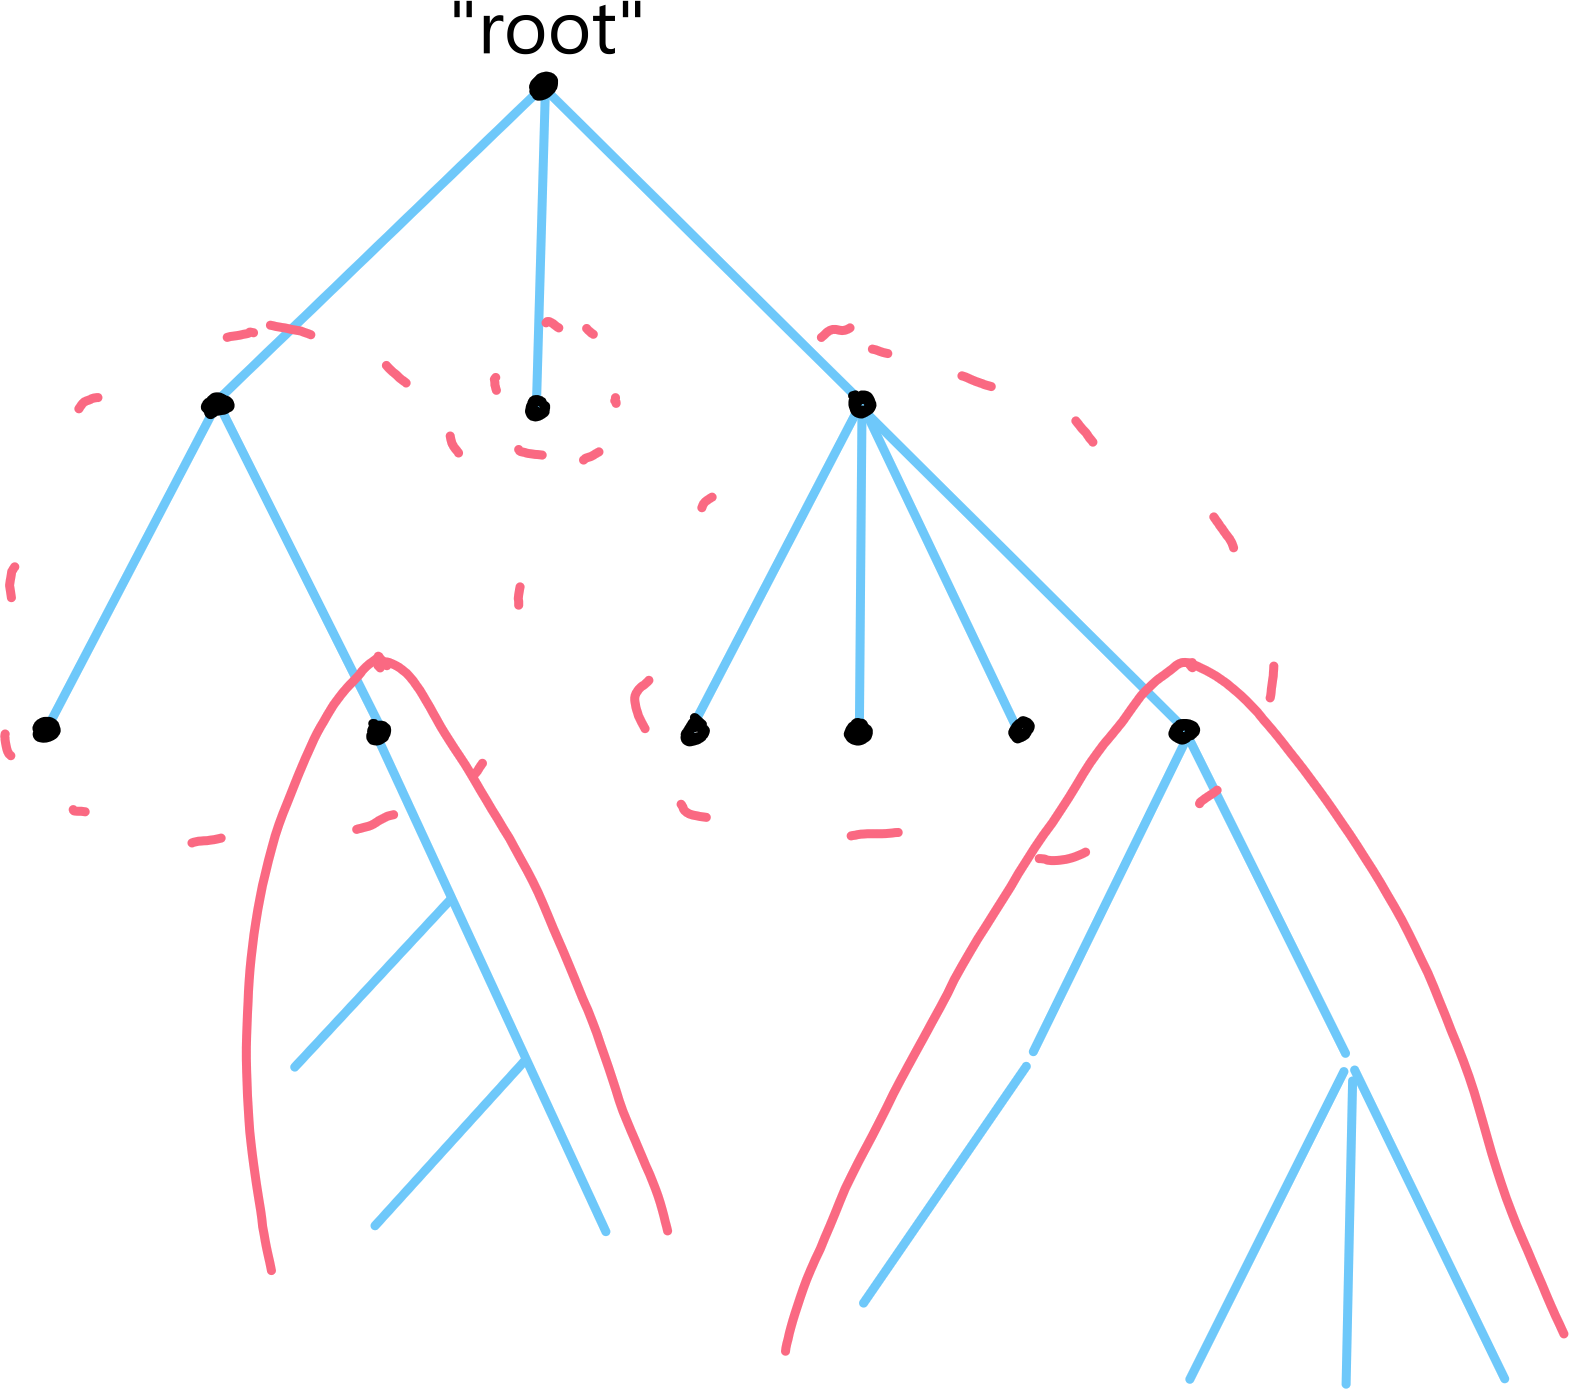
\includegraphics[width=10cm]{04-branch} 
\end{figure} 

\underline{Reduction}: Let $Z_n =$ be the number of individuals in generation $n$.
$Z_0 = 1$, $Z_1 \sim X$, $Z_{n + 1} = X_1^{(n)} + \dots + X_{Z_n}^{(n)}$ where $X_k^{(n)}$ are IID with distribution $X$ and independent of $Z_n$. 
\color{blue}``$X_k^{(n)} =$ number of children of kth individual in generation $n$.'' \color{black}

\begin{note}
    If $Z_n = 0 \implies Z_{n + 1} = Z_{n + 2} = \dots = 0$.
\end{note} 

\begin{theorem}
    $\mathbb{E}[Z_n] = (\mathbb{E}[X])^n$
\end{theorem} 

\begin{proof}
    $Z_{n + 1}$ is a random sum so $\mathbb{E}[Z_{n + 1}] = \mathbb{E}[X] \mathbb{E}[Z_n]$.
    By induction the result follows. 
\end{proof}

\begin{notation}
    $\mu = \mathbb{E}[X] \implies \mathbb{E}[Z_n] = \mu^n$.
\end{notation} 

\begin{notation} \label{not:branchpgf}
    Let $G$ be the PGF of $X$ and $G_n$ the PGF of $Z_n$.
\end{notation} 

\begin{theorem} \label{thm:branchpgf}
    $G_n(z) = G(\dots G(z) \dots)$\footnote{Sometimes written as $G^n(z)$, but this is confusing notation so we won't use it}.
\end{theorem} 

\begin{proof}
    $G_{n + 1}(z) = G_n(G(z))$ by \nameref{prp:randsum} and so result follows by induction.
\end{proof}

\begin{question}
    What is the probability the population has goes extinct?
\end{question} 

\begin{definition}[Extinction Probability by generation $n$]
    The probability that the population is extinct by generation $n$ is $q_n = \mathbb{P}(Z_n = 0)$.
\end{definition}

\begin{definition}[Extinction Probability]
    The probability that the population goes extinct is $q = \mathbb{P}(Z_n = 0 \text{ for any } n \geq 1)$, i.e. the population size is finite.
\end{definition}

\begin{note}
    $\{Z_n = 0\} \subseteq \{Z_{n + 1} = 0\}$ as $Z_n = 0 \implies Z_{n + 1} = 0$.
    Also $\{Z_n = 0 \text{ for any } n \geq 1\} = \bigcup_{n \geq 1} \{Z_n = 0\}$.
\end{note} 

\begin{theorem}
    $\mathbb{P}(Z_n = 0) \uparrow \mathbb{P}(\bigcup_{n \geq 1} \{Z_n = 0\})$\footnote{$\uparrow$ is convergence with an increasing sequence.}, i.e. $q_n \uparrow q$ as $n \to \infty$.
\end{theorem} 

\begin{proof}
    By \nameref{prp:continuity}.
\end{proof} 

There are 3 cases to consider
\begin{itemize}
    \item $\mu < 1$ - subcritical
    \item $\mu = 1$ - critical
    \item $\mu > 1$ - supercritical
\end{itemize} 

\color{blue} The degenerate case $\mathbb{P}(X = 1) = 1$ is boring so we exclude it. \color{black}

\begin{theorem}
    $q = 1 \iff \mu = \mathbb{E}[X] \leq 1$.\footnote{This does not hold in the degenerate case obviously.}
\end{theorem} 

\begin{remark} \color{blue} 
    Interesting that $q$ depends on $X$ only through $\mathbb{E}[X]$.
\end{remark} 

\underline{Interpretation}: Consider a pandemic spreading through a population, obviously it cannot infect infinite people.
Instead we take ``finite'' to mean e.g. 100 people are infected out of a large population and ``infinite'' might mean the model stops making sense/ a significant positive proportion are infected.

\begin{proof}[Baby Proof - (Subcritical)]
    \begin{align*}
        \mathbb{P}(Z_n \geq 1) &\leq \frac{\mathbb{E}[Z_n]}{1} \ \text{ by \nameref{clm:markov}} \\
        &= \mu^n \to 0.
    \end{align*} 
    For supercritical case, \color{red} note $\mathbb{E}[Z_n] \to \infty$ does \underline{not} imply $\mathbb{P}(Z_n = 0) \not\to 1$.
\end{proof} 

Recall $G$ is the PGF of $X$ and $G_n$ the PGF of $Z_n$, $q_n = \mathbb{P}(Z_n = 0) = G_n(0)$ and that $q$ is the extinction probability.

\begin{claim} \label{clm:branchpgf}
    $G(q) = q$.
\end{claim}

\begin{proof}[Proof 1.]
    $q_{n+1} = G(q_n)$ by \Cref{thm:branchpgf}, $q_n \to q$ and $G$ is continuous as it's a power series so $G(q_n) \to G(q)$ so $q = G(q)$ as $n \to \infty$.
\end{proof}

\begin{proof}[Proof 2 - LTP (revision of random sums)]
    Conditional on $Z_1 = k$, we get $k$ independent branching processes.

    \tikzset{every picture/.style={line width=0.75pt}} %set default line width to 0.75pt        
    
    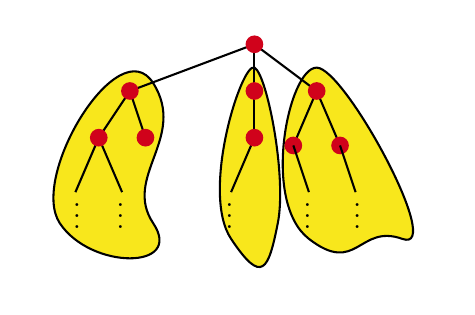
\begin{tikzpicture}[x=0.75pt,y=0.75pt,yscale=-0.75,xscale=0.75]
    %uncomment if require: \path (0,300); %set diagram left start at 0, and has height of 300
    
    %Shape: Polygon Curved [id:ds39756330989696687] 
    \draw  [fill={rgb, 255:red, 248; green, 231; blue, 28 }  ,fill opacity=1 ] (210,80) .. controls (232,115) and (190,140) .. (210,170) .. controls (230,200) and (170,200) .. (150,170) .. controls (130,140) and (188,45) .. (210,80) -- cycle ;
    %Shape: Polygon Curved [id:ds6379465750469737] 
    \draw  [fill={rgb, 255:red, 248; green, 231; blue, 28 }  ,fill opacity=1 ] (275,70) .. controls (283,74) and (296,140) .. (290,170) .. controls (284,200) and (280,210) .. (260,180) .. controls (240,150) and (267,66) .. (275,70) -- cycle ;
    %Shape: Polygon Curved [id:ds8073009612262341] 
    \draw  [fill={rgb, 255:red, 248; green, 231; blue, 28 }  ,fill opacity=1 ] (315,70) .. controls (333,70) and (398,190) .. (370,180) .. controls (342,170) and (341,204) .. (310,180) .. controls (279,156) and (297,70) .. (315,70) -- cycle ;
    %Straight Lines [id:da4966370314659285] 
    \draw    (275,55) -- (195,85) ;
    %Straight Lines [id:da012619115368816214] 
    \draw    (195,85) -- (175,115) ;
    %Straight Lines [id:da6584759199495862] 
    \draw    (315,85) -- (275,55) ;
    %Straight Lines [id:da6264172554803165] 
    \draw    (275,55) -- (275,85) ;
    %Straight Lines [id:da10191236924904246] 
    \draw    (275,85) -- (275,115) ;
    %Straight Lines [id:da8454343099013522] 
    \draw    (195,85) -- (205,115) ;
    %Straight Lines [id:da5191712973579519] 
    \draw    (275,115) -- (260,150) ;
    %Straight Lines [id:da2866173505227845] 
    \draw    (175,115) -- (160,150) ;
    %Straight Lines [id:da5251550145753905] 
    \draw    (175,115) -- (190,150) ;
    %Straight Lines [id:da7969351562542346] 
    \draw    (315,85) -- (300,120) ;
    %Straight Lines [id:da9516356439304474] 
    \draw    (315,85) -- (330,120) ;
    %Shape: Circle [id:dp2072526843406961] 
    \draw  [color={rgb, 255:red, 208; green, 2; blue, 27 }  ,draw opacity=1 ][fill={rgb, 255:red, 208; green, 2; blue, 27 }  ,fill opacity=1 ] (190,85) .. controls (190,82.24) and (192.24,80) .. (195,80) .. controls (197.76,80) and (200,82.24) .. (200,85) .. controls (200,87.76) and (197.76,90) .. (195,90) .. controls (192.24,90) and (190,87.76) .. (190,85) -- cycle ;
    %Shape: Circle [id:dp9783169345220857] 
    \draw  [color={rgb, 255:red, 208; green, 2; blue, 27 }  ,draw opacity=1 ][fill={rgb, 255:red, 208; green, 2; blue, 27 }  ,fill opacity=1 ] (325,120) .. controls (325,117.24) and (327.24,115) .. (330,115) .. controls (332.76,115) and (335,117.24) .. (335,120) .. controls (335,122.76) and (332.76,125) .. (330,125) .. controls (327.24,125) and (325,122.76) .. (325,120) -- cycle ;
    %Shape: Circle [id:dp4926704073297845] 
    \draw  [color={rgb, 255:red, 208; green, 2; blue, 27 }  ,draw opacity=1 ][fill={rgb, 255:red, 208; green, 2; blue, 27 }  ,fill opacity=1 ] (310,85) .. controls (310,82.24) and (312.24,80) .. (315,80) .. controls (317.76,80) and (320,82.24) .. (320,85) .. controls (320,87.76) and (317.76,90) .. (315,90) .. controls (312.24,90) and (310,87.76) .. (310,85) -- cycle ;
    %Shape: Circle [id:dp9137052205134757] 
    \draw  [color={rgb, 255:red, 208; green, 2; blue, 27 }  ,draw opacity=1 ][fill={rgb, 255:red, 208; green, 2; blue, 27 }  ,fill opacity=1 ] (295,120) .. controls (295,117.24) and (297.24,115) .. (300,115) .. controls (302.76,115) and (305,117.24) .. (305,120) .. controls (305,122.76) and (302.76,125) .. (300,125) .. controls (297.24,125) and (295,122.76) .. (295,120) -- cycle ;
    %Shape: Circle [id:dp7992097944836307] 
    \draw  [color={rgb, 255:red, 208; green, 2; blue, 27 }  ,draw opacity=1 ][fill={rgb, 255:red, 208; green, 2; blue, 27 }  ,fill opacity=1 ] (200,115) .. controls (200,112.24) and (202.24,110) .. (205,110) .. controls (207.76,110) and (210,112.24) .. (210,115) .. controls (210,117.76) and (207.76,120) .. (205,120) .. controls (202.24,120) and (200,117.76) .. (200,115) -- cycle ;
    %Shape: Circle [id:dp8305157135492074] 
    \draw  [color={rgb, 255:red, 208; green, 2; blue, 27 }  ,draw opacity=1 ][fill={rgb, 255:red, 208; green, 2; blue, 27 }  ,fill opacity=1 ] (170,115) .. controls (170,112.24) and (172.24,110) .. (175,110) .. controls (177.76,110) and (180,112.24) .. (180,115) .. controls (180,117.76) and (177.76,120) .. (175,120) .. controls (172.24,120) and (170,117.76) .. (170,115) -- cycle ;
    %Shape: Circle [id:dp9668393196026197] 
    \draw  [color={rgb, 255:red, 208; green, 2; blue, 27 }  ,draw opacity=1 ][fill={rgb, 255:red, 208; green, 2; blue, 27 }  ,fill opacity=1 ] (270,115) .. controls (270,112.24) and (272.24,110) .. (275,110) .. controls (277.76,110) and (280,112.24) .. (280,115) .. controls (280,117.76) and (277.76,120) .. (275,120) .. controls (272.24,120) and (270,117.76) .. (270,115) -- cycle ;
    %Shape: Circle [id:dp4143559387276672] 
    \draw  [color={rgb, 255:red, 208; green, 2; blue, 27 }  ,draw opacity=1 ][fill={rgb, 255:red, 208; green, 2; blue, 27 }  ,fill opacity=1 ] (270,55) .. controls (270,52.24) and (272.24,50) .. (275,50) .. controls (277.76,50) and (280,52.24) .. (280,55) .. controls (280,57.76) and (277.76,60) .. (275,60) .. controls (272.24,60) and (270,57.76) .. (270,55) -- cycle ;
    %Shape: Circle [id:dp6716716115264691] 
    \draw  [color={rgb, 255:red, 208; green, 2; blue, 27 }  ,draw opacity=1 ][fill={rgb, 255:red, 208; green, 2; blue, 27 }  ,fill opacity=1 ] (270,85) .. controls (270,82.24) and (272.24,80) .. (275,80) .. controls (277.76,80) and (280,82.24) .. (280,85) .. controls (280,87.76) and (277.76,90) .. (275,90) .. controls (272.24,90) and (270,87.76) .. (270,85) -- cycle ;
    %Straight Lines [id:da03905545740393146] 
    \draw    (300,120) -- (310,150) ;
    %Straight Lines [id:da03738266096433085] 
    \draw    (330,120) -- (340,150) ;
    
    % Text Node
    \draw (161,160) node    {$\vdots $};
    % Text Node
    \draw (189,160) node    {$\vdots $};
    % Text Node
    \draw (259,160) node    {$\vdots $};
    % Text Node
    \draw (309,160) node    {$\vdots $};
    % Text Node
    \draw (341,160) node    {$\vdots $};
    % Text Node
    \draw (234,90) node    {$\dotsc $};
    
    
    \end{tikzpicture}

    The total population is finite $\iff$ all subtrees\footnote{\color{blue} Each subtree has the same distribution as the original tree.} of \nth{1} generation are finite.
    \begin{align*}
        q &= \mathbb{P}(\text{finite}) \\
        &= \sum_{k \geq 0} \mathbb{P}(\text{all finite} \mid Z_1 = k) \mathbb{P}(Z_1 = k) \\
        &= \sum_{k \geq 0} [\mathbb{P}(\text{finite})]^k \mathbb{P}(Z_1 = k) \\
        &= \sum q^k \mathbb{P}(Z_1 = k) \\
        &= G(q). 
    \end{align*} 

    \underline{Facts about G}
    \begin{itemize}
        \item $G(0) = \mathbb{P}(X = 0) \geq 0$
        \item $G(1) = 1$
        \item $G'(1) = \mathbb{E}[X] = \mu$.
        \item $G$ is \underline{smooth}, all derivatives $\geq 0$ on $[0, 1)$ as all coefficients of the power series are non-negative.
    \end{itemize} 
 
    \tikzset{every picture/.style={line width=0.75pt}} %set default line width to 0.75pt        
    
    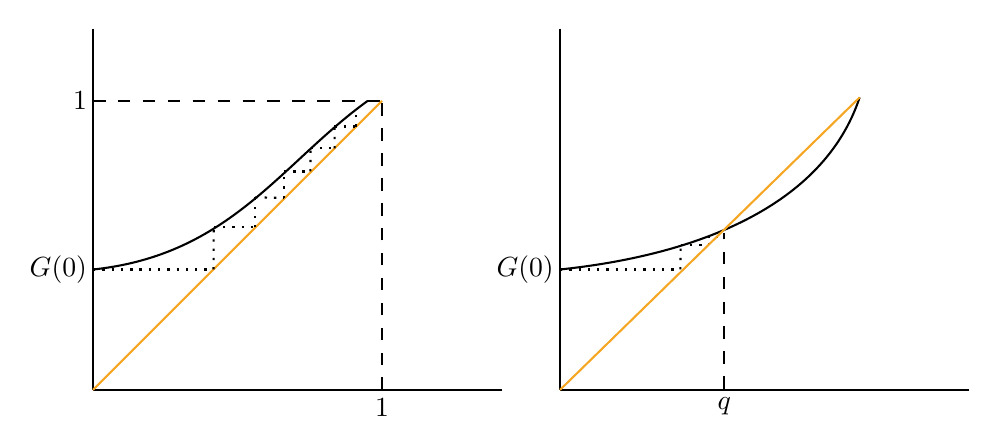
\begin{tikzpicture}[x=0.75pt,y=0.75pt,yscale=-0.75,xscale=0.75]
    %uncomment if require: \path (0,820); %set diagram left start at 0, and has height of 820
    
    %Straight Lines [id:da3566472400103051] 
    \draw    (77.07,60) -- (77.07,292) ;
    %Straight Lines [id:da30593282072011996] 
    \draw    (340,292) -- (77.07,292) ;
    %Straight Lines [id:da4498600243653825] 
    \draw  [dash pattern={on 4.5pt off 4.5pt}]  (77.07,106.4) -- (262.67,106.4) ;
    %Straight Lines [id:da23330676870406375] 
    \draw  [dash pattern={on 4.5pt off 4.5pt}]  (262.67,292) -- (262.67,106.4) ;
    %Straight Lines [id:da7917034040416375] 
    \draw [color={rgb, 255:red, 245; green, 166; blue, 35 }  ,draw opacity=1 ]   (262.67,106.4) -- (77.07,292) ;
    %Curve Lines [id:da28945061334157707] 
    \draw    (77.07,214.67) .. controls (165.23,205.39) and (197.71,146.61) .. (253.39,106.4) ;
    %Straight Lines [id:da5923563349362415] 
    \draw  [dash pattern={on 0.84pt off 2.51pt}]  (77.07,214.67) -- (154.4,214.67) ;
    %Straight Lines [id:da6561123702182479] 
    \draw  [dash pattern={on 0.84pt off 2.51pt}]  (154.4,214.67) -- (154.6,187.67) ;
    %Straight Lines [id:da11817016362725852] 
    \draw  [dash pattern={on 0.84pt off 2.51pt}]  (154.6,187.67) -- (181.34,187.67) ;
    %Straight Lines [id:da5269040164238137] 
    \draw  [dash pattern={on 0.84pt off 2.51pt}]  (181.34,187.67) -- (181.34,168.29) ;
    %Straight Lines [id:da277083738848787] 
    \draw  [dash pattern={on 0.84pt off 2.51pt}]  (181.34,168.29) -- (199.67,168.73) ;
    %Straight Lines [id:da16311358371686424] 
    \draw  [dash pattern={on 0.84pt off 2.51pt}]  (199.67,168.73) -- (199.67,151.71) ;
    %Straight Lines [id:da7565353729355639] 
    \draw  [dash pattern={on 0.84pt off 2.51pt}]  (199.67,151.71) -- (216.69,151.71) ;
    %Straight Lines [id:da1753488502260936] 
    \draw  [dash pattern={on 0.84pt off 2.51pt}]  (216.69,151.71) -- (216.76,136.87) ;
    %Straight Lines [id:da5142578403064464] 
    \draw  [dash pattern={on 0.84pt off 2.51pt}]  (216.76,136.87) -- (232.23,136.87) ;
    %Straight Lines [id:da6510626123810166] 
    \draw  [dash pattern={on 0.84pt off 2.51pt}]  (232.23,136.87) -- (232.14,122.83) ;
    %Straight Lines [id:da29923484937339095] 
    \draw  [dash pattern={on 0.84pt off 2.51pt}]  (232.14,122.83) -- (246.06,122.83) ;
    %Straight Lines [id:da34578049100722796] 
    \draw  [dash pattern={on 0.84pt off 2.51pt}]  (246.06,122.83) -- (246.06,112.01) ;
    %Straight Lines [id:da7302764276625526] 
    \draw    (377,60) -- (377,292) ;
    %Straight Lines [id:da7795005021532544] 
    \draw    (639.93,292) -- (377,292) ;
    %Straight Lines [id:da33689560520140405] 
    \draw  [dash pattern={on 4.5pt off 4.5pt}]  (482.61,291.28) -- (482.61,191.01) ;
    %Curve Lines [id:da3993780573627619] 
    \draw    (377,214.67) .. controls (465.16,205.39) and (546.33,174.03) .. (569.5,104.12) ;
    %Straight Lines [id:da575658635871469] 
    \draw  [dash pattern={on 0.84pt off 2.51pt}]  (377,214.67) -- (454.33,214.67) ;
    %Straight Lines [id:da272355400423417] 
    \draw  [dash pattern={on 0.84pt off 2.51pt}]  (454.33,214.67) -- (454.53,199.04) ;
    %Straight Lines [id:da2543476335628043] 
    \draw  [dash pattern={on 0.84pt off 2.51pt}]  (454.53,199.04) -- (472.58,199.04) ;
    %Straight Lines [id:da8309056535722565] 
    \draw  [dash pattern={on 0.84pt off 2.51pt}]  (472.58,199.04) -- (472.58,193.02) ;
    %Straight Lines [id:da05239577254419703] 
    \draw  [dash pattern={on 0.84pt off 2.51pt}]  (471.91,193.69) -- (477.93,193.69) ;
    %Straight Lines [id:da7959659183906378] 
    \draw [color={rgb, 255:red, 245; green, 166; blue, 35 }  ,draw opacity=1 ]   (569.5,104.12) -- (377,292) ;
    
    % Text Node
    \draw (262.67,295.4) node [anchor=north] [inner sep=0.75pt]    {$1$};
    % Text Node
    \draw (75.07,106.4) node [anchor=east] [inner sep=0.75pt]    {$1$};
    % Text Node
    \draw (75.07,214.67) node [anchor=east] [inner sep=0.75pt]    {$G( 0)$};
    % Text Node
    \draw (482.61,294.68) node [anchor=north] [inner sep=0.75pt]    {$q$};
    % Text Node
    \draw (375,214.67) node [anchor=east] [inner sep=0.75pt]    {$G( 0)$};
    \end{tikzpicture}\\
    The \nth{1} graph has gradient $< 1$ so only one solution at $q = 1$. \\
    In the \nth{2} graph, the gradient is $> 1$ so there is only one solution on $[0, 1)$ by IVT on $G(z) - z$.
\end{proof}

\begin{theorem}
    $q$, the extinction probability, is the \underline{minimal} solution to $z = G(z)$ in $[0, 1]$.\footnote{Assuming $\mathbb{P}(X = 1) \neq 1$.}
\end{theorem}

\begin{corollary}
    $q = 1 \iff \mu \leq 1$
\end{corollary} 

\begin{proof}
    Let $t$ be the minimal solution to $t = G(t)$.
    Reminder: $G$ is increasing.
    \begin{align*}
        t &\geq 0 \\
        \implies G(t) &\geq G(0) \\
        \implies G(G(t)) &\geq G(G(0)) \\
        \implies G(\dots G(t) \dots) &\geq G(\dots G(0) \dots) \\
        t &\geq q_n \\
        t &\geq q \ \text{ as } n \to \infty.
    \end{align*} 
    $q$ is a solution by Claim \ref{clm:branchpgf} and is bounded above by the minimal solution so $t = q$.
\end{proof}